% The official FRI template enables PDF/A metadata here. It is temporarily disabled because
% MiKTeX 25.12 currently ships mutually incompatible latex-lab/pdfmanagement package versions.
% Re-enable after the local TeX distribution update is fixed:
% \DocumentMetadata{pdfstandard=a-2b,pdfversion=1.7}
\documentclass[a4paper,12pt,twoside,openany]{book}

% -----------------------------------------------------------------------------
% Editable metadata. Replace the TODO values before submission.
% -----------------------------------------------------------------------------
\newcommand{\tauthor}{David Muhič}
\newcommand{\temail}{TODO@student.uni-lj.si}
\newcommand{\tmentor}{Branko Šter} % add academic title
\newcommand{\tsomentor}{Swarnendu Ghosh} % add academic title
\newcommand{\tinst}{Fakulteta za računalništvo in informatiko}
\newcommand{\tstopnja}{UNIVERZITETNI ŠTUDIJSKI PROGRAM PRVE STOPNJE\\RAČUNALNIŠTVO IN INFORMATIKA}
\newcommand{\tvrsta}{Diplomsko delo}

% The Slovene title is deliberately kept editable until it is approved.
\newcommand{\ttitle}{Kompleksna navigacija na podlagi spodbujevalnega učenja}
\newcommand{\ttitleEn}{Complex Navigation Based on Reinforcement Learning}
\newcommand{\tkeywords}{spodbujevalno učenje, vodenje rakete, ponovna uporabnost, simulacija, Unity}
\newcommand{\tkeywordsEn}{reinforcement learning, rocket control, reusable launch vehicle, simulation, Unity}

\newcommand{\tdescription}{TODO: Vstavite uradni opis teme iz sistema STUDIS.}
\newcommand{\tdescriptionEn}{TODO: Insert the approved English translation of the official STUDIS thesis description.}
\newcommand{\tzahvala}{TODO: Add acknowledgements.}
\newcommand{\tposvetilo}{}

\newcommand{\tpovzetek}{TODO: Slovene translation will be written after the English draft is approved.}
\newcommand{\tabstract}{%
Reusable-booster control combines translation, rotation, actuator limits, hardware faults, changing mass and environmental forces into a single control problem. This thesis presents a configurable simulator as a tool for studying this problem through reinforcement learning, with Proximal Policy Optimization (PPO) as its primary training algorithm.
The simulator gives users various controls over the experiment: they can configure their vehicle, set environmental conditions, select the task the vehicle should perform, customize the reward function and choose which telemetry to log for deeper analysis. They can then train a policy from scratch, initialize one from existing weights or evaluate a trained policy.
Three tasks have been demonstrated: fixed hover, moving-target hover tracking and physical four-leg landing. All 250 fixed-hover trials reached the 60-second evaluation horizon and converged to low speed, tilt and vertical error, while retaining a 4.77-metre mean planar offset; because no binary hover criterion was declared, this is reported as continuous evidence rather than a success rate. The simulator also supports actuator faults, variable environmental conditions and tower-catch landing, but these capabilities have not yet been experimentally validated.}

%%%%%%%%%%%%%%%%%%%%%%%%%%%%%%%%%%%%%%%%
% datoteka preambula.tex se uporablja v diploma-FRI-vzorec.tex
%%%%%%%%%%%%%%%%%%%%%%%%%%%%%%%%%%%%%%%%

\usepackage[T1]{fontenc}      % omogoča normalno kopiranje slovenskih črk
\usepackage{lmodern}
\usepackage[utf8]{inputenc}   % omogoča uporabo slovenskih črk kodiranih v formatu UTF-8
\usepackage[slovene,american]{babel}    % naloži, med drugim, slovenske naslove poglavij in delilne vzorce
\usepackage{microtype}         % boljša postavitev
\usepackage[pdftex]{graphicx}  % omogoča vlaganje slik različnih formatov
\usepackage{fancyhdr}          % poskrbi, na primer, za glave strani
\usepackage{amssymb}           % dodatni matematični simboli
\usepackage{amsmath}           % eqref, npr.
\usepackage{amsfonts}
\usepackage[hyphens]{url}
\usepackage{color}
\usepackage{soul}
\usepackage{subcaption}
\usepackage{booktabs}
\usepackage{tabularx}
\usepackage{longtable}
\usepackage{array}
\usepackage{float}
\usepackage{xcolor}
\usepackage{tikz}
\usetikzlibrary{positioning,arrows.meta,calc,fit}

% A restrained, colour-blind-friendly visual language used throughout the thesis.
% All figures remain editable in LaTeX and reproduce cleanly in grayscale.
\definecolor{rocketNavy}{HTML}{17324D}
\definecolor{rocketBlue}{HTML}{3E6F9E}
\definecolor{rocketTeal}{HTML}{25877A}
\definecolor{rocketAmber}{HTML}{D8952A}
\definecolor{rocketRed}{HTML}{B84A4A}
\definecolor{rocketInk}{HTML}{26343F}
\definecolor{rocketGrid}{HTML}{D9E2E8}
\definecolor{rocketPaper}{HTML}{F5F8FA}
\tikzset{
  rocketbox/.style={draw=rocketNavy!38,fill=rocketPaper,rounded corners=3pt,
    thick,align=center,inner sep=7pt,text=rocketInk},
  rocketarrow/.style={-{Latex[length=2.3mm]},thick,draw=rocketBlue},
  chartgrid/.style={draw=rocketGrid,thin},
  chartaxis/.style={-{Latex[length=2mm]},draw=rocketInk,thick}
}
\usepackage{algorithm}
\usepackage{algpseudocode}
\usepackage[
  backend=biber,
  style=numeric,
  sorting=nty,
]{biblatex}

\addbibresource{references.bib}
\graphicspath{{./podporno/}{./figures/}}

%%%%%%%%%%%%%%%%%%%%%%%%%%%%%%%%%%%%%%%%
%  enote (decimalna vejica)
%%%%%%%%%%%%%%%%%%%%%%%%%%%%%%%%%%%%%%%%

\usepackage{siunitx}
\sisetup{
  output-decimal-marker = {,}
}

%%%%%%%%%%%%%%%%%%%%%%%%%%%%%%%%%%%%%%%%
%  URLs
%%%%%%%%%%%%%%%%%%%%%%%%%%%%%%%%%%%%%%%%

% najprej podtaknemo opcijo za deljenje URL-jev pri vezajih
\PassOptionsToPackage{hyphens}{url}

% nato naložimo hyperref z vsemi tvojimi nastavitvami
\usepackage[
    pdftex, 
    unicode,                % Podpora za slovenske znake v PDF kazalu/metapodatkih
    colorlinks=true,
    citecolor=black, 
    filecolor=black,
    linkcolor=black, 
    urlcolor=black,
    pdfproducer={LaTeX}, 
    pdfcreator={LaTeX}
]{hyperref}


% \newcommand{\ttitle}{Vzorec diplomskega dela}
% \newcommand{\ttitleEn}{Diploma thesis template}
% \newcommand{\tsubject}{\ttitle}
% \newcommand{\tsubjectEn}{\ttitleEn}
% \newcommand{\tauthor}{Matjaž Kralj}
% \newcommand{\tkeywords}{računalnik, računalnik, računalnik}
% \newcommand{\tkeywordsEn}{computer, computer, computer}

%%%%%%%%%%%%%%%%%%%%%%%%%%%%%%%%%%%%%%%%
%  HYPERREF SETUP
%%%%%%%%%%%%%%%%%%%%%%%%%%%%%%%%%%%%%%%%
\hypersetup{pdftitle={\ttitle}}
\hypersetup{pdfsubject=\ttitleEn}
\hypersetup{pdfauthor={\tauthor}}
\hypersetup{pdfkeywords=\tkeywordsEn}

%%%%%%%%%%%%%%%%%%%%%%%%%%%%%%%%%%%%%%%%
% postavitev strani
%%%%%%%%%%%%%%%%%%%%%%%%%%%%%%%%%%%%%%%%

\addtolength{\marginparwidth}{-20pt} % robovi za tisk
\addtolength{\oddsidemargin}{40pt}
\addtolength{\evensidemargin}{-40pt}

\renewcommand{\baselinestretch}{1.3} % ustrezen razmik med vrsticami
\setlength{\emergencystretch}{3em}   % allows graceful line breaks around long identifiers
\setlength{\headheight}{15pt}        % potreben prostor na vrhu
\renewcommand{\chaptermark}[1]%
{\markboth{\MakeUppercase{\thechapter.\ #1}}{}} \renewcommand{\sectionmark}[1]%
{\markright{\MakeUppercase{\thesection.\ #1}}} \renewcommand{\headrulewidth}{0.5pt} \renewcommand{\footrulewidth}{0pt}
\fancyhf{}
\fancyhead[LE,RO]{\sl \thepage}
%\fancyhead[LO]{\sl \rightmark} \fancyhead[RE]{\sl \leftmark}
\fancyhead[RE]{\sc \tauthor}              % dodal Solina
\fancyhead[LO]{\sc Diplomska naloga}     % dodal Solina

\newcommand{\BibLaTeX}{{\sc Bib}\LaTeX}
\newcommand{\BibTeX}{{\sc Bib}\TeX}

%%%%%%%%%%%%%%%%%%%%%%%%%%%%%%%%%%%%%%%%
% naslovi
%%%%%%%%%%%%%%%%%%%%%%%%%%%%%%%%%%%%%%%%

\newcommand{\autfont}{\Large}
\newcommand{\titfont}{\LARGE\bf}
\newcommand{\clearemptydoublepage}{\newpage{\pagestyle{empty}\cleardoublepage}}
\setcounter{tocdepth}{1}        % globina kazala

%%%%%%%%%%%%%%%%%%%%%%%%%%%%%%%%%%%%%%%%
% konstrukti
%%%%%%%%%%%%%%%%%%%%%%%%%%%%%%%%%%%%%%%%
\newtheorem{izrek}{Izrek}[chapter]
\newtheorem{trditev}{Trditev}[izrek]
\newenvironment{dokaz}{\emph{Dokaz.}\ }{\hspace{\fill}{$\Box$}}

%%%%%%%%%%%%%%%%%%%%%%%%%%%%%%%%%%%%%%%%
% define medatata
%%%%%%%%%%%%%%%%%%%%%%%%%%%%%%%%%%%%%%%%
\def\Title{\ttitle}
\def\Author{\tauthor, \temail}
\def\Subject{\ttitleEn}
\def\Keywords{\tkeywordsEn}

%%%%%%%%%%%%%%%%%%%%%%%%%%%%%%%%%%%%%%%%
% \convertDate converts D:20080419103507+02'00' to 2008-04-19T10:35:07+02:00
%%%%%%%%%%%%%%%%%%%%%%%%%%%%%%%%%%%%%%%%
\def\convertDate{%
  \getYear
}

{\catcode`\D=12
  \gdef\getYear D:#1#2#3#4{\edef\xYear{#1#2#3#4}\getMonth}
}
\def\getMonth#1#2{\edef\xMonth{#1#2}\getDay}
\def\getDay#1#2{\edef\xDay{#1#2}\getHour}
\def\getHour#1#2{\edef\xHour{#1#2}\getMin}
\def\getMin#1#2{\edef\xMin{#1#2}\getSec}
\def\getSec#1#2{\edef\xSec{#1#2}\getTZh}
\def\getTZh +#1#2{\edef\xTZh{#1#2}\getTZm}
\def\getTZm '#1#2'{%
  \edef\xTZm{#1#2}%
  \edef\convDate{\xYear-\xMonth-\xDay T\xHour:\xMin:\xSec+\xTZh:\xTZm}%
}

%\expandafter\convertDate\pdfcreationdate

%%%%%%%%%%%%%%%%%%%%%%%%%%%%%%%%%%%%%%%%
% get pdftex version string
%%%%%%%%%%%%%%%%%%%%%%%%%%%%%%%%%%%%%%%%
\newcount\countA
\countA=\pdftexversion
\advance \countA by -100
\def\pdftexVersionStr{pdfTeX-1.\the\countA.\pdftexrevision}

%%%%%%%%%%%%%%%%%%%%%%%%%%%%%%%%%%%%%%%%
% XMP data
%%%%%%%%%%%%%%%%%%%%%%%%%%%%%%%%%%%%%%%%
\usepackage{xmpincl}
%\includexmp{pdfa-1b}

%%%%%%%%%%%%%%%%%%%%%%%%%%%%%%%%%%%%%%%%
% PDF metadata is written by hyperref above. Keeping a second \pdfinfo block
% creates duplicate dictionary keys in current pdfTeX versions.
%%%%%%%%%%%%%%%%%%%%%%%%%%%%%%%%%%%%%%%%

%%%%%%%%%%%%%%%%%%%%%%%%%%%%%%%%%%%%%%%%
% vključevanje programske kode
%%%%%%%%%%%%%%%%%%%%%%%%%%%%%%%%%%%%%%%%
\usepackage[hypcap=false]{caption}
% The working draft does not require an external syntax-highlighting process.
\usepackage{listings}
\definecolor{svetlo-siva}{gray}{0.96}
\lstset{basicstyle=\ttfamily\footnotesize,backgroundcolor=\color{svetlo-siva},
  frame=lines,breaklines=true,numbers=left,numberstyle=\tiny}

% izsek za slovenščino
\addto\captionsslovene{%
  \renewcommand{\lstlistingname}{Izsek kode}%
}

% izsek za angleščino
\addto\captionsenglish{%
  \renewcommand{\lstlistingname}{Code Snippet}%
}

%%%%%%%%%%%%%%%%%%%%%%%%%%%%%%%%%%%%%%%%
% znaki za copyright stran
%%%%%%%%%%%%%%%%%%%%%%%%%%%%%%%%%%%%%%%%

\newcommand{\CcImageCc}[1]{%
  
\includegraphics[scale=#1]{cc_cc_30.pdf}%
}
\newcommand{\CcImageBy}[1]{%
  
\includegraphics[scale=#1]{cc_by_30.pdf}%
}
\newcommand{\CcImageSa}[1]{%
  
\includegraphics[scale=#1]{cc_sa_30.pdf}%
}

%%%%%%%%%%%%%%%%%%%%%%%%%%%%%%%%%%%%%%%%
\usepackage[autostyle=true]{csquotes} % za narekovaje

% Če želite uporabljati klasične slovenske „narekovaje“ (so enaki nemškim):
\DeclareQuoteAlias{german}{slovene}
% Če pa želite imeti koničaste tipkarske »narekovaje« pa zgornjo vrstico odstranite.


% Long, visible placeholders make incompleteness impossible to mistake for a result.
\newenvironment{thesistodo}{\begin{quote}\color{red!70!black}\textbf{TODO before submission:} }{\end{quote}}
\newcommand{\projectname}{RocketSim}

\begin{document}
\input{podporno/naslovnestrani}

\mainmatter
\selectlanguage{american}
\sisetup{output-decimal-marker={.}}
\pagestyle{fancy}

\chapter{Introduction}
\label{ch:introduction}

The idea for this project came from watching a reusable booster land safely on a small landing pad. I could not help but be impressed by the precision and elegance with which such a powerful vehicle could maneuver. I immediately began thinking about how I might approach the design of such a complex system.

My first ideas were crude: manually encoding a collection of conditional rules, building a controller based on altitude, attitude and velocity, or even attempting to control the vehicle manually. A possible approach emerged during an artificial-intelligence class taught by Dr Bosnič, who presented a student project in which an agent trained using reinforcement learning controlled a swordsman in combat. This was a turning point: the control problem did not necessarily have to be solved by hand. I began to suspect that a machine could discover a more precise control strategy than I could design manually.

To test this idea, I chose Unity, an engine with which I already had experience, and used Unity ML-Agents to connect the simulation to a Python trainer
\cite{juliani2020mlagents,unitymlagentsrepo}. In April 2026, I built an initial prototype: a cylinder driven by one oversized, instantly responding engine. It consumed no fuel, had no drag or wind, and ignored other aerodynamic forces. It handled observations, actions, rewards, termination logic and visual effects in a single \texttt{FalconAgent} script. Its purpose was narrow: to determine whether the training loop could produce a policy capable of controlling a simplified booster. Although training was not straightforward, the prototype ultimately succeeded at a basic landing task, providing initial evidence that the approach was viable.

That initial success was encouraging, but it solved only a simplified version of the landing problem with an unrealistically capable vehicle. A realistic reusable-booster landing would require the controller to manage several additional layers of complexity. From a distance, the maneuver looks simple: descend towards the landing spot, remain upright and arrive at near-zero velocity. In practice, these objectives compete. The vehicle must simultaneously regulate position, velocity and attitude while thrust is limited, actuators respond with delay, fuel consumption changes the mass properties and aerodynamic forces vary with wind.

As these constraints were introduced, the experiment became increasingly tangled. Each new feature created dependencies between the policy, vehicle configuration, task logic and simulator state. It became difficult to modify one part without affecting another or to distinguish policy failures from simulator defects. The system therefore had to be restructured and modularized, with its components separated so that they could evolve independently and remain observable.

The original plan was to train separate controllers for several mission phases, but this scope proved too broad. The work therefore narrowed to landing while the software around it became more ambitious: the single-purpose prototype evolved towards a configurable platform for defining vehicles, tasks, training settings and evaluation conditions.

The thesis therefore focuses on the development of a configurable rocket-control simulator rather than solely on a single landing policy. Proximal Policy Optimization (PPO) is used as the primary training algorithm to validate the system; it is not intended as a comparison of learning algorithms. Three tasks have been demonstrated in the current system: fixed hover, moving-target hover tracking and physical four-leg landing. Support for actuator faults, variable environmental conditions, alternative vehicle configurations and tower-catch landing is also implemented, but these capabilities have not yet been experimentally validated.

\section{Problem statement}

The practical problem is not merely to make one policy land. It is to construct an experimental platform in which vehicle, atmosphere, task, learning and telemetry settings can be changed without silently invalidating the results. An RL policy can exploit reward definitions and simulator defects just as readily as it can learn the intended behaviour. Consequently, the simulator must make its assumptions explicit, preserve the exact configuration used for each run, and provide an evaluation path that is independent of the trainer's own progress signal.

The work addresses three research questions:

\begin{description}
	\item[RQ1] How can a Unity-based rocket-control simulator be structured so that configurable
	RL experiments remain modular and reproducible?
	\item[RQ2] Can PPO policies trained in the simulator perform fixed hover, moving-target hover
	tracking and physical four-leg landing under a predefined deterministic evaluation protocol?
	\item[RQ3] Which reward, physical-modeling and software-integration failures arise during
	development, and which design changes make them observable or prevent their recurrence?
\end{description}

\section{Contributions}

The principal contributions are:

\begin{enumerate}
	\item a configurable six-degree-of-freedom rigid-body simulation with modular engines, grid
	fins, reaction-control thrusters, landing legs, fuel-dependent mass properties, atmosphere
	and wind;
	\item immutable session snapshots that separate editable UI state from the configuration
	consumed by running simulation areas;
	\item task-owned observation, reward, termination and curriculum definitions for fixed hover,
	moving-target hover tracking and physical four-leg landing;
	\item versioned training artifacts, compatibility checks, telemetry and deterministic
	evaluation under fixed curriculum bands; and
	\item empirical case studies showing measurable learning across most of the moving-target
	hover-tracking curriculum and the complete physical four-leg landing curriculum, including
	the remaining deterministic deployment boundary and the sequence of simulator and reward
	changes that made physical landing learnable.
\end{enumerate}

\section{Thesis structure}

Chapter~\ref{ch:background} introduces the control and RL concepts. Chapters~\ref{ch:scope}
and~\ref{ch:architecture} define the method and software design. Chapters~\ref{ch:physics}
and~\ref{ch:learning} describe the physical and learning models. Chapter~\ref{ch:development}
records the main engineering challenges. Chapters~\ref{ch:evaluation} and~\ref{ch:results}
specify the evaluation and report available results. Chapter~\ref{ch:limitations} discusses the
validity limits and future work, and Chapter~\ref{ch:conclusion} concludes the thesis.
\chapter{Background and Related Work}
\label{ch:background}

The decision to use reinforcement learning changed the problem rather than removing it. Instead
of writing a complete controller by hand, I now had to build an environment in which useful
control could be learned. Four ideas shaped that environment: the physical demands of powered
descent, the reinforcement-learning formulation, the behaviour of PPO, and the distinction
between progress during training and performance during evaluation.

\section{Reusable-booster control}

A Falcon-class booster has nine first-stage engines, four deployable landing legs and four grid
fins, and burns liquid oxygen and rocket-grade kerosene \cite{spacex2025falcon}. These details
provided a useful scale and suggested which components the simulator would eventually need.
They did not make the implemented vehicle a certified Falcon~9 model or digital twin: public
dimensions and propulsion data establish plausible proportions, while the controller learns
only from the physical model defined in Chapter~\ref{ch:physics}.

The landing problem is difficult because translation and rotation cannot be solved separately.
Tilting the vehicle redirects thrust to correct a horizontal error, but simultaneously reduces
the vertical component needed to slow the descent. The amount of available control then changes
with throttle limits, actuator delay, fuel consumption, atmosphere and contact with the ground.
What appears visually to be one smooth manoeuvre is therefore a sequence of tightly coupled
decisions made under a shrinking margin for error.

Powered-descent guidance is often formulated as an optimal-control problem. Convexification can
transform relevant constraints into a form suitable for onboard optimization
\cite{acikmese2007convex}. Neural methods can instead approximate a control law after observing
many solved or sampled trajectories \cite{sanchez2018dnncontrol}, while deep reinforcement
learning has been applied directly to six-degree-of-freedom planetary landing with continuous
actions and randomized initial conditions \cite{gaudet2020landing}. This thesis shares the
control objective of that work, but asks a different engineering question: how can an
interactive Unity environment remain configurable and reproducible while the vehicle, task and
reward are still evolving?

\section{Reinforcement learning model}

An episodic Markov decision process is described by states $s_t$, actions $a_t$, transition
dynamics, rewards $r_t$ and a discount factor $\gamma$. A policy
$\pi_\theta(a_t\mid s_t)$ with parameters $\theta$ selects actions so as to maximize the expected
discounted return
\begin{equation}
  J(\theta)=\mathbb{E}_{\pi_\theta}\!\left[\sum_{t=0}^{T-1}\gamma^t r_t\right].
  \label{eq:return}
\end{equation}
The simulator does not provide the policy with a perfect physical state. It constructs an
observation vector $o_t$ from normalized relative kinematics, attitude and actuator state, so
the learned controller is more precisely written $\pi_\theta(a_t\mid o_t)$.

This formulation makes the reward function especially important. A human description such as
``land softly near the centre'' is not available to the optimizer; only the numerical reward
and termination rules are. A collection of individually sensible terms can therefore describe
an unintended strategy more profitably than the intended one. Potential-based shaping can
preserve an optimal policy under specific conditions \cite{ng1999policy}, but this project also
uses bounded physical costs, event rewards and terminal outcomes. Those terms have to be audited
empirically. The early policy that hovered just above the ground illustrates why: a small reward
paid repeatedly eventually outweighed the one-off value of actually landing.

\section{Proximal Policy Optimization}

PPO was selected because Unity ML-Agents supports it directly and because the rocket primarily
uses continuous control. PPO alternates between collecting trajectories under an existing
policy and improving that policy through a clipped surrogate objective
\cite{schulman2017ppo}. With probability ratio
\begin{equation}
  r_t(\theta)=\frac{\pi_\theta(a_t\mid o_t)}
  {\pi_{\theta_{\mathrm{old}}}(a_t\mid o_t)},
\end{equation}
the clipped objective is
\begin{equation}
  L^{\mathrm{CLIP}}(\theta)=
  \mathbb{E}_t\left[\min\left(r_t(\theta)\hat A_t,
  \operatorname{clip}(r_t(\theta),1-\epsilon,1+\epsilon)\hat A_t\right)\right],
  \label{eq:ppo}
\end{equation}
where $\hat A_t$ estimates the advantage of an action. Clipping limits the incentive for one
update to move too far from the policy that produced the data.

That stability is useful, but it does not protect the experiment from a missing observation, an
incorrect force or a reward loophole. PPO will optimize the task it is given, including any
mistake in that task. The experiments therefore use it as a consistent way to validate the
simulator rather than as a claim that PPO is the best algorithm for rocket landing. Unity
ML-Agents exchanges trajectories with the Python trainer, and the resulting multilayer
perceptron is exported to ONNX for inference inside Unity. No camera input is used; all policy
inputs are numerical observations derived from the simulated state.

\section{Curricula and evaluation}

The complete landing and tracking tasks were too broad to present to an untrained policy at
once. The simulator therefore represents difficulty with a scalar $d\in[0,1]$ and interpolates
between initial and final parameter ranges,
\begin{equation}
  x(d)=(1-d)x_{\mathrm{initial}}+d x_{\mathrm{full}}.
  \label{eq:curriculum-interpolation}
\end{equation}
As performance improves, the curriculum increases spawn distances, initial velocities or the
strictness of success thresholds. The sampled difficulty is frozen for the duration of an
episode, or for one target in the tracking task, so that the rules cannot change midway through
an attempt. Easier replay episodes remain in the distribution to reduce forgetting.

Curriculum progress answers whether the trainer is making the task harder; it does not answer
how reliable the exported policy is. Progress depends on recent training samples, adaptive
counters and stochastic actions. This became important in L11, where exact-full-difficulty
training success was much higher than deterministic evaluation success. For that reason,
evaluation fixes the seed, tests explicit difficulty bands and records every episode separately.

Binary success is reported with a Wilson score interval. For $n$ trials, observed proportion
$\hat p$ and normal quantile $z=1.96$, the interval is
\begin{equation}
\frac{\hat p+z^2/(2n)\ \pm\ z\sqrt{\hat p(1-\hat p)/n+z^2/(4n^2)}}
     {1+z^2/n}.
\label{eq:wilson}
\end{equation}
It remains well behaved near zero and one, where a symmetric normal approximation is misleading.

Deep-RL results can also vary across training seeds and implementation details
\cite{henderson2018matters,agarwal2021precipice}. Because the available computation and schedule
allowed only one principal training seed per task, the numerical results in this thesis validate
the simulator workflow and describe these particular policies. They are not a statistically
general comparison between algorithms.

\chapter{Scope and Method}
\label{ch:scope}

\section{From a demonstration to an engineering objective}

The first cylinder answered the original feasibility question: reinforcement learning could
produce a basic landing behaviour. It could not answer whether that result would survive a
change of vehicle, reward, actuator or simulator version. The engineering objective therefore
shifted from producing one successful policy to producing a desktop simulator in which an
experiment could be configured, repeated and inspected.

In the resulting workflow, a user defines the vehicle, environment, task, reward, learning run
and telemetry before launching one or more independent simulation areas. The same application
supports PPO training, ONNX inference, deterministic evaluation and component-level tests. A
completed run should retain the configuration that produced it, and a policy whose observation
or action interface no longer matches the vehicle should be rejected before inference begins.

The simulator eventually grew beyond what could be evaluated within one bachelor thesis. The
experimental scope was therefore reduced to a sequence of three increasingly demanding tasks:
holding a fixed hover, tracking relocated hover targets, and landing on four physical legs.
Alternative vehicle configurations, wind and injected actuator faults remain implemented
capabilities, but they are not presented as validated results. External-arm capture is treated
as a separate future task rather than being added to an already broad landing study.

\section{Development method}

Development followed the same loop throughout the project:

\begin{enumerate}
  \item add or modify one physical, actuator or task component;
  \item test its direction, limits and feasibility independently of learning;
  \item train a policy and inspect trajectories, episode outcomes and telemetry;
  \item identify the simulator defect, reward loophole or control limitation revealed by the
  new behaviour;
  \item move configuration and responsibility into a clearer module when the change exposed
  unwanted coupling; and
  \item preserve the resulting configuration as a new run or immutable revision before
  continuing.
\end{enumerate}

This method emerged because training alone was a poor debugging instrument. A bad learning
curve could mean that the task was too difficult, but it could also mean that drag pointed in
the wrong direction or that the requested spawn velocity was never applied. I therefore added
what the interface calls \emph{hardware tests}: component-level experiments inside Unity that
isolate the simulated hardware from the policy. No physical rocket hardware was built or
tested. These checks answer questions such as whether drag opposes air-relative motion, whether
an engine respects its spool rate, and whether the available thrust can arrest the selected
descent.

The important part of the loop is that an unexpected policy is treated as evidence. It is first
reproduced and measured, then used to decide what the next run should change. Chapter~\ref{ch:development}
applies this method to the L1--L11 landing campaign.

\section{Separating capability from evidence}

As the simulator gained features, it became easy to confuse an available checkbox with an
evaluated contribution. To prevent that, this thesis uses three evidence classes. A
\emph{completed evaluation} executes its predefined episode count and fixed seed without manual
interruption. A \emph{preliminary diagnostic} can reveal useful behaviour but is too small or
incomplete for a reliability claim. A \emph{capability} exists in the code or UI but has not yet
been evaluated under the thesis protocol.

The \texttt{HoverFixed}, moving-target hover and L11 landing policies have completed their
planned evaluation episode counts. L10 is retained as a completed landing baseline because
comparing it with L11 shows what changed after the actuator and reward redesign. Fixed hover is
reported through continuous state and control metrics because its evaluator still has no binary
success rule; completing 250 horizons is not silently relabelled as 100\% task success. Wind,
faults and vehicle-configuration comparisons remain capabilities. These labels follow each
result into Chapters~\ref{ch:evaluation}--\ref{ch:limitations}.

\section{Reproducibility boundary}

Each reported run is identified by its run ID, session revision, environment and trainer seed,
training configuration, exported model and evaluation summary. This record is the final step of
the development loop: it connects a plotted result back to the exact experiment that produced
it. The public repository URL and commit cannot be filled in truthfully until the working tree
is frozen, because the current Git HEAD does not include uncommitted simulator changes.

\begin{thesistodo}
  Freeze the submission revision, publish the repository, and replace the repository and commit
  placeholders in Appendix~\ref{app:reproducibility}. Do this only after the working tree is
  stable, so that the published identity matches the submitted implementation.
\end{thesistodo}

\chapter{Simulator Architecture}
\label{ch:architecture}

The prototype could afford to keep its state inside one agent because it represented one
vehicle and one task. That stopped working as soon as the right-side configuration panel was
introduced. A value could now exist in three forms: what the user was editing, what the
simulator had accepted, and what an already running episode was using. Resolving that ambiguity
became the central architectural problem. The final design follows the life of an experiment
from an editable idea to a frozen result.

\section{The simulator as an experimental product}

The application is organized around one user journey. The user configures a vehicle and task,
checks the derived policy interface, launches training or inference, and inspects the resulting
telemetry and artifacts. Figure~\ref{fig:product-workflow} shows this path. The final arrow back
to configuration is important: most useful changes in this project were responses to evidence
from the previous run.

\begin{figure}[htbp]
  \centering
  \begin{tikzpicture}[node distance=0.32cm]
    \node[rocketbox,text width=0.175\textwidth,minimum height=2.55cm] (configure) {
      \textcolor{rocketBlue}{\Large\textbf{1}}\\[2pt]
      \textbf{Configure}\\[3pt]
      \footnotesize vehicle, task, rewards, environment, trainer, faults and telemetry};
    \node[rocketbox,text width=0.175\textwidth,minimum height=2.55cm,right=of configure] (freeze) {
      \textcolor{rocketBlue}{\Large\textbf{2}}\\[2pt]
      \textbf{Check \& freeze}\\[3pt]
      \footnotesize validate feasibility, derive the policy schema and create an immutable session};
    \node[rocketbox,text width=0.175\textwidth,minimum height=2.55cm,right=of freeze] (execute) {
      \textcolor{rocketTeal}{\Large\textbf{3}}\\[2pt]
      \textbf{Execute}\\[3pt]
      \footnotesize train with PPO, run ONNX inference, evaluate or perform component tests};
    \node[rocketbox,text width=0.175\textwidth,minimum height=2.55cm,right=of execute] (inspect) {
      \textcolor{rocketAmber}{\Large\textbf{4}}\\[2pt]
      \textbf{Inspect}\\[3pt]
      \footnotesize review trajectories, reward terms, outcomes, checkpoints and manifests};
    \draw[rocketarrow] (configure) -- (freeze);
    \draw[rocketarrow] (freeze) -- (execute);
    \draw[rocketarrow] (execute) -- (inspect);
    \draw[-{Latex[length=2.3mm]},thick,dashed,draw=rocketAmber]
      ([yshift=-4mm]inspect.south) -- ++(0,-0.45) -| ([yshift=-4mm]configure.south)
      node[pos=0.47,below,font=\footnotesize,text=rocketInk]{evidence informs the next revision};
  \end{tikzpicture}
  \caption{The experiment workflow. Editable settings become a validated, immutable session
  before any simulation area or trainer consumes them.}
  \label{fig:product-workflow}
\end{figure}

The configuration panel mirrors the decisions needed for an experiment: vehicle hardware,
task and curriculum, rewards and termination, environment, learning, faults and telemetry.
Built-in presets provide a usable starting point, but their values remain editable and a user
can save new presets. The same path can therefore create a lightweight single-engine vehicle or
a Falcon~9-inspired multi-engine vehicle without placing vehicle-specific logic inside a task.

This workflow also separates four questions that the prototype used to blur together. Is the
configuration syntactically valid? Is the requested manoeuvre physically feasible? Does a
trained model still match the selected hardware? Does it actually succeed? Validation addresses
the first, component tests support the second, schema checks protect the third, and only a
frozen evaluation can answer the fourth.

\section{From editable settings to immutable state}

The first major redesign established a one-way configuration flow. The UI edits a
\texttt{SimulationSessionDraft}. Starting a run validates that draft and converts it into an
immutable \texttt{SimulationSessionSnapshot}. The \texttt{SimulationRunCoordinator} then creates
the requested simulation areas, and each \texttt{SimulationAreaHost} receives its own runtime
copy. From that point onward, the rocket and agent read the snapshot rather than the UI.

This boundary was added after scripts began reading and changing shared component values
directly. It was no longer clear whether a number on screen was a proposed value, a corrected
value after validation, or the value already used by training. Snapshotting turns ``start'' into
an explicit state transition. It also makes the accepted configuration serializable and gives
the manifest a stable object to hash.

The snapshot contains five main sections:

\begin{description}
  \item[Vehicle] geometry, mass, fuel, engine layout and actuator parameters;
  \item[Environment] task, atmosphere, wind, curricula, inference mode, seeds and faults;
  \item[Objective] task-specific rewards, shaping ranges and terminations;
  \item[Learning] behaviour schema, PPO settings and resume policy; and
  \item[Telemetry] enabled streams, sample rate and output location.
\end{description}

Validation derives dependent quantities and reports infeasible combinations before launch. A
warning can still be overridden for an intentional sandbox experiment, but that override is
stored in the session. It no longer disappears as an undocumented click.

\section{Breaking apart the original agent}

Once configuration had a clear owner, runtime behaviour needed the same treatment. The original
\texttt{FalconAgent} handled observations, actions, actuation, rewards, spawning, termination and
visual effects. It was convenient while the rocket was a cylinder; later, almost every change
touched the same file and created side effects elsewhere.

The current \texttt{RocketAssembly} builds the rigid body and selected components. Engines,
grid fins, reaction-control thrusters and landing legs own their local state, central systems
combine forces and mass properties, and the agent supplies normalized commands. Agent logic is
split by responsibility into lifecycle, observations, actuators, guidance, spawning, rewards,
telemetry and scenario-specific behaviour. Separate services own session lifecycle, area
creation and trainer startup. Some large partial classes remain, but new task behaviour now has
a defined location instead of another switch in a global script.

\section{A policy interface that follows the vehicle}

Modular hardware created the next problem: changing the vehicle also changes what the policy
must observe and control. Manually updating ML-Agents behaviour parameters became both tedious
and unsafe. The simulator now derives those dimensions from the accepted snapshot.

The base observation vector contains 21 values describing relative target kinematics,
orientation and global vehicle state. Engine timing adds five shared observations, followed by
eight values for each independently controlled engine: throttle, two gimbal coordinates, four
one-hot run states and a constraint timer. Leg landing adds four foot-contact values. Grid-fin,
RCS and separate engine-enable control add further component-dependent observations or actions.

For $N_e$ engine channels, $N_f$ fins and $N_r$ RCS channels, the continuous action size is
\begin{equation}
  n_a = (3+I_{\mathrm{enable}})N_e+N_f+N_r,
  \label{eq:actions}
\end{equation}
where $I_{\mathrm{enable}}\in\{0,1\}$. Policy outputs are bounded and then mapped to throttle,
gimbal or component-specific physical limits.

Shape alone is not enough to guarantee compatibility. Two observation vectors can have the same
length while assigning different meanings to their elements. The model artifact therefore
stores the derived schema, and resume or inference checks compare observation count, action
count, component layout, behaviour name, trainer type and network settings. This contract was
added after simulator changes made older policies unsafe to reuse and, in some cases, corrupted
the intended continuity of a run.

\section{Versioned runs instead of overwritten experiments}

The same problem appeared over time as well as across vehicles. A promising run often needed a
longer step budget, but resuming it by overwriting the old configuration erased the conditions
that had produced earlier checkpoints. The run format now keeps a top-level manifest and mutable
runtime progress alongside numbered, immutable revision directories. Every revision stores its
session JSON, launch manifest and trainer YAML; logs, checkpoints and the final ONNX model remain
associated with the run ID.

The launch manifest records the Python executable and package versions, GPU, seed, launch mode
and SHA-256 digest of the session. Curriculum counters are stored separately in runtime state
because they change while training proceeds. In this way a continuation can advance the same
policy without rewriting the identity of the experiment that created it. The L10 and L11
histories in Chapters~\ref{ch:development} and~\ref{ch:results} rely on this distinction.

\section{Starting Unity and the trainer in the right order}

The final architectural failure appeared before an episode had even begun. ML-Agents originally
opened its connection as soon as Unity entered Play mode, while the configurable rocket prefabs
had not yet been created. The trainer could therefore connect to an incomplete or unintended
agent.

The coordinator now validates the snapshot, creates every requested simulation area and only
then enables the ML-Agents behaviour. Dummy prefabs satisfy Unity editor references without
registering an agent; actual runtime prefabs are created after the configuration is known. The
same coordinator derives the final policy schema before allowing the run to start.

Physics advances every \SI{0.01}{s}. The standard decision period is three physics steps, so the
policy supplies a new command every \SI{0.03}{s}, while actuator state, forces and the contact
solver continue to update between decisions. This ordering keeps high-frequency physical
dynamics independent of the neural-network inference frequency and completes the path from an
editable experiment to a running, reproducible simulation.

\chapter{Physical and Actuator Model}
\label{ch:physics}

The first prototype needed only gravity and thrust. That was enough to test the learning loop,
but every step toward a reusable-booster-shaped vehicle exposed another missing interaction.
Fuel changed the mass, grid fins required airflow, airflow required atmosphere and wind, and a
landing could not be judged without modelling individual feet and post-contact motion. The
physical model grew in that order. Its purpose is to create a coherent control problem, not to
claim flight-level fidelity.

\section{Rigid-body foundation and changing mass}

Unity integrates a six-degree-of-freedom rigid body. Let position be $\mathbf p$, velocity
$\mathbf v$, body angular velocity $\boldsymbol\omega$, mass $m$ and inertia tensor
$\mathbf I$. Translational and rotational motion conceptually follow
\begin{align}
  m\dot{\mathbf v} &= \mathbf F_T+\mathbf F_A+m\mathbf g, \\
  \mathbf I\dot{\boldsymbol\omega}+
  \boldsymbol\omega\times(\mathbf I\boldsymbol\omega) &=
  \boldsymbol\tau_T+\boldsymbol\tau_A+\boldsymbol\tau_R,
\end{align}
where the subscripts denote thrust, aerodynamic and RCS contributions. The simulator calculates
forces, application points, mass and inertia; Unity performs numerical integration and contact
resolution.

The Falcon-inspired reference body uses radius \SI{1.83}{m}, height \SI{41.2}{m}, dry mass
\SI{22200}{kg} and maximum propellant mass \SI{400000}{kg}. These are configurable nominal
values rather than a complete accounting of real vehicle hardware. The early cylinder kept a
constant mass, which meant the same throttle always produced the same acceleration. Once fuel
consumption was introduced, the combined centre of mass became
\begin{equation}
  \mathbf r_{\mathrm{cm}}=\frac{\sum_i m_i\mathbf r_i}{\sum_i m_i}.
\end{equation}
Approximate component inertias are combined with the parallel-axis theorem. Propellant behaves
as a changing rigid mass; liquid slosh is outside the model.

\section{From still air to a repeatable environment}

Grid fins made airflow unavoidable. The simulator first needed density and air-relative
velocity before it could calculate any useful aerodynamic control. Air density follows the
exponential approximation
\begin{equation}
  \rho(h)=\rho_0 k_\rho \exp\!\left(-\frac{h}{H}\right),
  \label{eq:density}
\end{equation}
where $h$ is altitude, $H$ is a scale height and $k_\rho$ is a user-selected multiplier. A
configurable horizontal wind vector is subtracted from vehicle velocity,
$\mathbf v_a=\mathbf v-\mathbf v_{\mathrm{wind}}$, and an optional low-order gust varies that
vector over time.

The intention is controlled disturbance, not weather simulation. Direction randomization and a
fixed seed make wind experiments repeatable, but the model has no altitude profile, turbulence
spectrum or correlated three-dimensional gust field. A wind setting therefore proves that the
force path exists; it does not by itself prove that a policy is wind-robust.

\section{Discovering that drag must work in both directions}

The first drag implementation looked plausible during descent but behaved incorrectly when the
rocket moved upward. The error came from losing the sign of axial velocity. The current model
decomposes air-relative velocity into axial and lateral components and writes axial drag as
\begin{equation}
  \mathbf F_{D,a}=-\tfrac12\rho C_{D,a}A_a
  v_a\lvert v_a\rvert\,\hat{\mathbf e}_a,
  \label{eq:axialdrag}
\end{equation}
with nominal $C_{D,a}=0.30$. The product $v_a\lvert v_a\rvert$ preserves direction, so the force
opposes both upward and downward motion.

Broadside drag uses nominal coefficient $C_{D,s}=1.0$, projected side area and lateral velocity.
It is applied at an approximate centre of pressure and therefore also produces torque. A small
base-drag term acts during tail-first descent. Separating these components made sign and scale
errors easier to test than a single global drag coefficient, although the result remains a
low-order model without Mach-dependent tables, compressibility or plume interaction.

\section{Grid fins and the limits of visual geometry}

Once body drag behaved consistently, the grid fins could contribute control forces. Their
response scales with dynamic pressure
\begin{equation}
  q=\tfrac12\rho\lVert\mathbf v_a\rVert^2.
\end{equation}
Each fin has a configurable envelope, deflection limit and slew rate. The nominal envelope is
\SI{1.59}{m} by \SI{1.23}{m}, with \SI{0.30}{m} thickness and an effective lift scale of 0.5.

An early version treated too much of that envelope as a solid aerodynamic plate. A real grid fin
contains open lattice, but resolving that flow is beyond the simulator. The model instead uses
the visible envelope for geometry and reduces its idealized response with the lift scale. This
does not reproduce lattice aerodynamics; it records the approximation explicitly and lets the
user vary it.

\section{Propulsion, fuel and actuator timing}

Adding more realistic engines changed the problem more than simply changing maximum thrust. An
engine command contains throttle and two gimbal coordinates. For each active engine,
\begin{equation}
  \mathbf F_T=T_{\max}\,k_T(h)\,u_T\,\hat{\mathbf e}_{\mathrm{gimbal}},
\end{equation}
where $u_T$ respects the configured minimum throttle and $k_T(h)$ approximates the change from
sea-level to vacuum thrust using the pressure ratio from Equation~\eqref{eq:density}. A sandbox
preset, for example, uses maximum sea-level thrust \SI{845}{kN}, specific impulse \SI{282}{s},
minimum throttle 0.39 and maximum gimbal angle \SI{7}{\degree}.

Fuel flow is calculated from
\begin{equation}
  \dot m_f=-\frac{T}{I_{\mathrm{sp}}g_0}.
  \label{eq:massflow}
\end{equation}
The effective $I_{\mathrm{sp}}$ is adjusted approximately with pressure. Neither this adjustment
nor the thrust interpolation is presented as a proprietary engine model.

The first engine responded instantly, allowing the policy to create control strategies that no
physical actuator could follow. Throttle spool, gimbal slew, startup delay, shutdown transient,
minimum run time and restart cooldown were introduced to close that gap. These constraints later
became part of the learning story themselves: strict timing made useful behaviour difficult to
discover in L8, while relaxed timing exposed excessive cycling and motivated L9--L11.

\section{From contact to a stable landing}

Touching the ground was initially enough to end an episode. That definition allowed one-foot
contacts, hard impacts and unstable rocking to appear successful. The final landing model exposes
four individual foot contacts and records first-contact velocity, tilt, angular rate, maximum
impulse, rebound height, stable-hold time, feet outside the pad and structural strikes. The
episode can therefore distinguish reaching the ground from completing a stable landing.

RCS channels follow the same modular pattern: they apply bounded forces and consume a separate
propellant budget using Equation~\eqref{eq:massflow}. The nominal thruster provides
\SI{750}{N}, has \SI{70}{s} specific impulse and respects a minimum \SI{0.10}{s} pulse.

Ground response still comes from Unity colliders and a general-purpose contact solver. The
simulator does not model crushing, detailed leg compliance, soil, structural deformation or
plume--ground interaction. A successful landing in this thesis therefore means success under
the documented collider geometry and thresholds, not proof that a real vehicle would survive.

\section{Verifying one layer before training the next}

Each addition created a new opportunity for motion that looked believable while being wrong. I
therefore used component-level tests for zero-wind drag direction, upward and downward motion,
vacuum and sea-level thrust scaling, fuel depletion, gimbal and throttle rates, RCS pulse timing,
centre-of-mass movement and leg-contact classification. These tests checked deterministic
properties before a policy was trained against them.

Training then acted as a second form of pressure testing. A policy repeats any profitable defect
far more consistently than a manual user. When a learned strategy violated the intended physics,
the behaviour was reduced to a component test and corrected there. This sequence---implement,
isolate, train and inspect---connected the physical model back to the development method in
Chapter~\ref{ch:scope}.

\chapter{Tasks, Rewards and Learning System}
\label{ch:learning}

The physical model defines what the rocket can do; the task definition determines what it is
asked to learn. In the prototype, those two concerns were mixed inside \texttt{FalconAgent}.
That was manageable for one landing experiment, but adding hover and target tracking created
conflicting spawn rules, rewards and termination conditions. The learning system was therefore
reorganized around task ownership before the final policies were trained.

\section{Making each task own its objective}

Every scenario now owns a versioned \texttt{ScenarioObjectiveConfig}. It contains the reward
magnitudes, shaping scales and termination parameters that give numerical meaning to that task.
The runtime applies the sign of costs, so values exposed in the UI remain nonnegative magnitudes;
a value of zero disables a term.

The distinction between continuous and one-off rewards became important after early policies
learned to wait for repeated payment. Continuous shaping values are defined as rates and
multiplied by the physics timestep. Contact events and terminal outcomes are emitted once. The
evaluation sequence is also fixed: measure the physical state, build the task context, calculate
shaping, add event and terminal terms, record the breakdown, and only then end the episode. A
terminal event can no longer disappear because another component terminated the episode first.

This organization did not make reward design automatic. It made each assumption visible and
allowed a reward change to become a versioned experimental decision rather than a hidden code
edit.

\section{Putting unlike physical quantities on a common scale}

Position error, speed and attitude are expressed in different units and ranges. Combining their
raw values made coefficients difficult to interpret, so many shaping terms use exponential
closeness
\begin{equation}
  E(x;s)=\exp\!\left(-\frac{\lvert x\rvert}{\lvert s\rvert}\right),
  \label{eq:exp01}
\end{equation}
where the user-visible scale $s$ describes how quickly the value decreases as error $x$ grows.
A general continuous reward rate can then be written
\begin{equation}
  \dot r = \sum_i w_i^+ E(e_i;s_i)-\sum_j w_j^- C_j,
  \qquad r_t=\dot r\,\Delta t+r_{\mathrm{event}}+r_{\mathrm{terminal}}.
  \label{eq:reward-general}
\end{equation}
The $w$ values are configurable magnitudes and each contribution can be logged separately. A
large total return can therefore be traced back to the behaviour that generated it instead of
being treated as proof that the policy is good.

\section{Fixed hover: learning to remain still}

Fixed hover isolates the most basic powered-flight question: can the policy keep the vehicle
near one point without touching the ground or flying away? The rocket starts near
\SI{50}{m} and is asked to settle near a target at \SI{30}{m}. Its reward combines altitude and
planar proximity, uprightness, low translational speed and low angular rate, with optional costs
for motion, effort and time.

This apparently simple task exposed one of the earliest reward loopholes. When similar proximity
terms were used for landing, hovering just above the surface accumulated more reward than ending
the episode with a touchdown. The policy was not refusing to land; the numerical objective had
made waiting more valuable. That behaviour led to the separation of rates, events and terminal
outcomes used by every later task.

A standard hover evaluation lasts \SI{60}{s}. The evaluator reports duration, position,
velocity, attitude and fuel but has no predeclared binary success threshold. The completed
\texttt{HoverFixed} evaluation is therefore reported through its physical distributions and
termination outcomes, not converted into a success percentage after the fact.

\section{Moving-target hover: separating travel from settling}

Once a policy could remain near one point, target tracking added a transition between stable
states. An evaluation episode begins with one hover target and relocates it twice after capture.
Each target must be reached and held within \SI{35}{s}; the curriculum increases the relocation
radius and tightens the capture limits.

A single proximity reward was not enough for both parts of this behaviour. Far from the target,
the useful action is to close distance at a sensible speed. Near it, the same speed becomes a
liability and the policy should settle. The task therefore has an approach phase, which rewards
closure, direction and useful speed, and a settle phase, which rewards centre proximity and calm
horizontal, vertical and rotational motion. Moving away, loitering and excessive speed can be
penalized. Capture is a timed event defined by bounded position and motion, not by crossing a
distance threshold for one frame.

This two-phase design became a useful bridge to landing. Both tasks require the policy to travel
while far away and change priorities as the terminal region approaches.

\section{Physical leg landing: rewarding the whole mission}

Landing adds the final elements missing from tracking: a descent profile, irreversible contact
and a requirement to remain supported afterwards. A height-dependent reference speed is based on
\begin{equation}
  v_{z,\mathrm{goal}}(h)=-k_v\sqrt{2g\max(h,0)},
  \label{eq:descent-profile}
\end{equation}
where curriculum-dependent fraction $k_v$ controls how aggressively the vehicle should descend.
In flight, the objective can use horizontal closure, profile error, uprightness, near-target
speed, angular rate, control effort and time. At the surface, it distinguishes first contact,
hard impact, rebound, support by four feet and stable touchdown.

Runs L2--L11 progressively changed the relationship between those terms. The decisive rule in
the final objective is that mission efficiency is calculated only after a successful landing.
Fuel use, restarts and additional engine ignitions can then distinguish two successful solutions,
but a failing policy cannot improve its outcome by switching everything off and giving up. The
behaviours that led to this rule are followed chronologically in
Section~\ref{sec:landing-iterations}.

Safety after contact is not delegated entirely to the learned policy. Any external impact locks
propulsion, off-pad impact ends immediately, and pad contact remains active long enough to
measure rebound, supported feet and stable hold. Reward is thus a signal used to discover the
behaviour, while evaluation success is a separate conjunction of physical conditions.

\section{Keeping the learning algorithm constant}

The tasks and simulator changed repeatedly, so the principal experiments kept one PPO
configuration instead of adding hyperparameter search as another source of variation.
Table~\ref{tab:ppo} lists the configuration shared by the completed tracking and L11 landing
runs. It should be read as an implementation choice, not as evidence that these values are
optimal.

\begin{table}[htbp]
  \centering
  \caption{PPO configuration for \texttt{HoverTrackSimple3} and \texttt{L11}.}
  \label{tab:ppo}
  \begin{tabular}{ll@{\qquad}ll}
    \toprule
    Parameter & Value & Parameter & Value \\
    \midrule
    Batch size & 4096 & Buffer size & 40960 \\
    Learning rate & $2\times10^{-4}$, linear & PPO clip $\epsilon$ & 0.2 \\
    Entropy $\beta$ & 0.01 & GAE $\lambda$ & 0.98 \\
    Epochs/update & 6 & Discount $\gamma$ & 0.9995 \\
    Hidden units & 512 & Hidden layers & 3 \\
    Time horizon & 1024 & Maximum steps & 30M tracking; 100M landing \\
    Checkpoint interval & 500,000 & Trainer seed & 1 \\
    \bottomrule
  \end{tabular}
\end{table}

The recorded environment used Python 3.10.12, ML-Agents 1.1.0, PyTorch 2.1.0 with CUDA 12.1,
and an NVIDIA GeForce RTX 4070 SUPER. The Unity project used Unity 6000.4.1f1 and ML-Agents
package 4.0.2. Neither principal run used fins, RCS or wind. Tracking used one engine channel,
30 observations and four continuous actions; L11 used three independent engines, 52
observations and 12 continuous actions. With the learning method fixed, the remaining changes
can be interpreted through the task, actuator and simulator revisions described next.

\chapter{Development and Engineering Challenges}
\label{ch:development}

\section{From prototype to simulator}

Development began in early April 2026 with the smallest experiment that could fail usefully: a
cylinder, one oversized engine and a policy asked to reach the ground slowly. By the middle of
April it could perform a basic landing. That result justified continuing, but every simplifying
assumption was still visible. The engine had no realistic minimum throttle, vehicle mass never
changed, and one \texttt{FalconAgent} script owned nearly the entire simulation.

The next step was not one large jump to realism. I replaced assumptions one at a time and let
each addition reveal the next missing layer. Moving to Falcon-class dimensions led to multiple
engines, grid fins and RCS. Grid fins were meaningless without airflow, so drag and atmosphere
followed. Wind then required air-relative velocity, while fuel consumption required changing
mass and inertia. Finally, spool, slew and engine timing prevented the policy from treating the
actuators as instantaneous mathematical commands.

Those physical additions also changed the policy interface. Manually maintaining ML-Agents
observation and action sizes became error-prone, so a launch manager began deriving the schema
and creating parallel areas. That exposed a startup-order bug: ML-Agents connected before valid
runtime rockets existed. Solving it produced the dummy/actual-prefab sequence described in
Chapter~\ref{ch:architecture}.

The largest transition came with the right-side configuration panel. Parameters that had lived
beside the code using them now had to travel from an editable UI into a running experiment. This
forced the snapshot architecture. Adding hover, tracking and landing then forced a second split,
because spawn distributions, rewards, curricula, terminations and evaluation criteria could no
longer remain global switches inside one agent. By this point, the project had changed from a
landing demonstration into the configurable experiment system described in the previous three
chapters.

\section{Challenge 1: reward loopholes}

Reward development produced the clearest examples of why the simulator had to become observable.
A coefficient could look reasonable during manual testing and remain apparently successful for
millions of steps, until the policy discovered a repeated action sequence with a better return.
The most important behaviours were:

\begin{itemize}
  \item hovering near the ground instead of landing because proximity rewards continued to
  accrue;
  \item touching down with only one foot while satisfying an overly broad contact condition;
  \item switching off thrust and dropping when future return appeared worse than termination;
  \item remaining nearly inactive when movement costs outweighed progress; and
  \item flipping or forcing a collision to end an unfavourable episode early.
\end{itemize}

At first I responded by changing coefficients or adding special cases. That worked for one
behaviour and usually created another. The more useful interpretation was that each policy had
found a counterexample to the written reward specification. The long-term response was to expose
rates, events, terminal values, scales and thresholds in the scenario configuration, log their
individual contributions, and make termination order explicit. This does not prevent a poor
reward, but it makes the reason for a high return inspectable and allows controlled changes
without rewriting task code.

\section{Leg-landing problem-solving campaign}
\label{sec:landing-iterations}

The numbered L1--L11 series turned that lesson into a repeatable process. I started a new
iteration only after inspecting the previous policy in the simulator and in episode- and
step-level telemetry. Each run therefore begins with a concrete question left by the one before
it. Because duration, reward scale, actuator timing and curriculum difficulty changed, their raw
returns are not a controlled algorithm benchmark. Their value lies in the chain of evidence:
what failed, how the cause was isolated, and whether the next intervention removed it.

\begin{figure}[htbp]
  \centering
  \begin{tikzpicture}[
      node distance=0.35cm,
      phase/.style={draw=rocketNavy!35,rounded corners=3pt,align=center,text width=0.198\textwidth,
        minimum height=2.2cm,inner sep=5pt,font=\small,text=rocketInk},
      arrow/.style={-{Latex[length=2.2mm]},thick,draw=rocketBlue}]
    \node[phase,fill=rocketRed!7] (p1) {\textbf{L1--L4}\\Infrastructure, spawn physics and termination\\
      \emph{Make a physical attempt preferable to a cheap reset}};
    \node[phase,fill=rocketAmber!10,right=of p1] (p2) {\textbf{L5--L7}\\Contact quality and reward economics\\
      \emph{Make a soft, centred touchdown preferable to a crash}};
    \node[phase,fill=rocketTeal!9,right=of p2] (p3) {\textbf{L8--L9}\\Learnability and actuator timing\\
      \emph{Bootstrap landing, then restore constraints}};
    \node[phase,fill=rocketBlue!8,right=of p3] (p4) {\textbf{L10--L11}\\Efficiency and generalization\\
      \emph{Reward the outcome and test the full range}};
    \draw[arrow] (p1) -- (p2);
    \draw[arrow] (p2) -- (p3);
    \draw[arrow] (p3) -- (p4);
  \end{tikzpicture}
  \caption{The four phases of the L1--L11 landing campaign. Each phase begins with a policy or
  infrastructure failure and ends with a narrower unsolved problem.}
  \label{fig:landing-phases}
\end{figure}

\footnotesize
\begin{longtable}{p{0.055\textwidth}p{0.245\textwidth}p{0.27\textwidth}p{0.30\textwidth}}
  \caption{Landing campaign at a glance. The table gives the decision made after each run; the
  evidence and comparisons are developed in the phase narratives below.}
  \label{tab:landing-iterations}\\
  \toprule
  Run & Failure exposed & Decisive change & Result or next question \\
  \midrule
  \endfirsthead
  \toprule
  Run & Failure exposed & Decisive change & Result or next question \\
  \midrule
  \endhead
  L1 & Trainer never connected. & Clear the occupied Unity worker. & Infrastructure failure;
  no policy was tested. \\
  L2 & The rocket spawned without its prescribed downward velocity. & Apply velocity only after
  the rigid body becomes dynamic. & Escape disappeared as an easy interpretation of the task. \\
  L3 & The policy reached the pad, then crashed at about \SI{40}{m/s}. & Remove time pressure and
  extend impact severity beyond its low cap. & Touchdown became preferable to a fast reset. \\
  L4 & A vehicle could approach the pad and then leave after an off-pad collision. & Lock
  propulsion and classify the first external collision immediately. & The surface could no
  longer be used as a powered recovery manoeuvre. \\
  L5 & Almost every episode touched down, but most were hard or waited off-centre. & Add settled
  off-centre termination and stronger stability shaping. & The next problem became reward
  ordering, not contact frequency. \\
  L6 & A hard crash was cheaper than a careful miss. & Rebalance terminal outcomes and expose
  additive readiness components. & The economics improved, but navigation progress still leaked. \\
  L7 & Descending increased ``readiness'' even while lateral error grew. & Remove the altitude
  gate derivative from navigation progress. & The reward finally measured motion toward the
  centre. \\
  L8 & The full actuator delay made useful landing behaviour difficult to discover. & Temporarily
  ease startup, minimum-run and cooldown timing. & Robust landing emerged, together with roughly
  30 ignitions per success. \\
  L9 & Rapid engine cycling synthesized thrust below the minimum. & Restore part of the timing
  constraint and warm-start from L8. & Cycling fell, but efficiency and engine choice remained
  weak. \\
  L10 & Directly prescribing an engine would overfit the solution. & Start fresh and reward
  efficiency only after successful touchdown. & 151/250 fixed-band successes; full difficulty
  and cycling remained unsolved. \\
  L11 & One-engine continuous descent was still physically awkward. & Lower minimum throttle and
  strengthen success-only cycling cost. & 212/250 successes, including 18/50 at full difficulty;
  mean restarts fell to 1.56. \\
  \bottomrule
\end{longtable}
\normalsize

\subsection{L1--L4: make the episode physically meaningful}

The first phase prevented the policy from optimizing simulator and termination defects. L1
never began because the communication worker was occupied. L2 then appeared to learn quickly:
mean return improved from about $-18.7$ to $-17.2$, the vehicle centred to roughly
\SI{0.64}{m}, ignited all three engines and climbed out of the episode in about \SI{3.6}{s}.
This was not landing progress. The policy had found the cheapest reset, and the simulator had
silently removed the prescribed 10--\SI{18}{m/s} initial downward velocity.

After staged velocity application in L3, the policy could no longer begin from rest. It learned
to navigate near the pad and remain upright, but then converted the next reward defect into a
fast vertical crash. The hard-touchdown severity term had a low cap, while every additional
second still incurred cost. Removing that time pressure and extending severity in L4 made
physical contact more attractive. Inspection then revealed a different safety gap: vehicles
that lost control after approaching the pad could continue thrusting after an off-pad impact.
The response was a physical propulsion lockout and immediate classification on every first
external collision.

\subsection{L5--L7: make safe touchdown cheaper than failure}

Once almost every trajectory reached the surface, the target moved from contact quantity to
contact quality. L5 exposed two post-contact loopholes. A rocket could rock between feet for
several seconds before becoming stable, or remain calm just outside the success radius until a
discounted timeout. The settled off-centre termination added for L6 removed the second behaviour,
but L6 regressed to 1.6\% late-window success because the reward ordering was wrong: a fast hard
contact was much cheaper than a carefully controlled miss.

L7 corrected the ordering and made readiness additive rather than a product that became zero if
one component was poor. At equal 10--13M budgets, success rose from 1.23\% in L6 to 8.81\% in L7.
Near-ground tilt fell from \SI{5.89}{\degree} to \SI{2.98}{\degree}, angular rate from
\SI{25.2}{\degree\per\second} to \SI{9}{\degree\per\second}, and vertical contact speed from
\SI{8.88}{m/s} to \SI{7.50}{m/s}. Yet only 34\% of sampled trajectories moved toward the pad
centre. Step telemetry finally identified the cause: positive ``readiness'' was recorded on
about 78\% of steps because descending increased the altitude gate even when lateral error grew.

\subsection{L8--L9: separate learnability from realism}

L8 removed the altitude derivative from the potential and temporarily shortened engine startup,
minimum-run and cooldown delays. This was a deliberate curriculum over actuator dynamics: the
goal was first to make navigation, braking and four-foot contact discoverable. At the same
10--13M budget, L8 achieved 82.4\% success versus L7's 8.8\%. Recent successful L8 landings
reduced an initial \SI{20.1}{m} pad distance to \SI{1.41}{m}, contacted at \SI{2.26}{m/s} and
\SI{1.13}{\degree} tilt, and shut down propulsion correctly after impact.

The easier actuator also exposed a new strategy: nearly 30 ignitions per success. L9 restored
part of the timing constraint while initializing from L8. At matched 55--65\% difficulty, L9
slightly improved non-replay success and reduced hard touchdowns and restarts, but used more
fuel and missed the centre more often. Above \SI{50}{m}, more than 77\% of powered samples still
used all three engines. Thus timing continuation reduced cycling without producing the desired
single-engine navigation mode.

\subsection{L10--L11: reward the mission, then test its boundary}

L10 deliberately did not prescribe which engine to use. It started from fresh weights and paid
an efficiency term only after successful touchdown. Fuel, restart-equivalent fuel and additional
first ignitions affected this outcome term, while failures could not improve return by shutting
down early. Training was extended from 30M to 50M and finally 79.63M steps as the curriculum
continued to advance. Chapter~\ref{ch:results} shows that the same policy improved its landing
quality under increasingly difficult starts, although full-difficulty evaluation remained
outside the learned distribution.

L11 tested that hypothesis in a fresh 100M-step run. Minimum throttle was lowered from 57\% to
49.9\%, while startup delay, shutdown transient, minimum run and restart cooldown were set to
\SI{0.45}{s}, \SI{0.20}{s}, \SI{1.5}{s} and \SI{2.0}{s}. The lower minimum thrust made a longer
single-engine descent feasible; the timing constraints and larger success-only restart
equivalent made rapid cycling unattractive without rewarding failures for switching off.

The curriculum reached 100\% and stayed there. In the frozen 250-episode evaluation, L11
completed 212 stable landings, including 18 of 50 at exact full difficulty. Mean engine restarts
fell from L10's 18.46 to 1.56 per episode and mean first-contact vertical speed fell from
\SI{3.02}{m/s} to \SI{1.33}{m/s}. Extending the same run from 90M to 100M steps produced a
smaller but measurable final improvement: overall success rose from 82.8\% to 84.8\% and
full-difficulty success from 30\% to 36\%. The final policy therefore resolved most of the
cycling problem and produced the first successes at the previously unsolved boundary, while
leaving a narrower
vertical-braking and deployment-consistency problem for future work.

\section{Challenge 2: aerodynamics and physics}

The landing campaign was not only a reward-design exercise. Some policies exposed mistakes in
the world they were learning from. I had no previous experience building a rocket-physics system,
and the most dangerous errors were not spectacular failures but plausible-looking forces with
the wrong meaning. Axial drag worked during descent but pointed incorrectly during upward motion;
the first grid-fin model gave too much authority because it treated an open lattice too much like
a solid surface.

Watching training revealed the symptoms, but component tests made them reproducible. That led to
the layered model in Chapter~\ref{ch:physics}: force components are separated, dimensional
quantities and coefficients are exposed, and tests check direction and bounds where practical.
Where high-fidelity data was unavailable, I chose an explicit approximation rather than hidden
precision. The simulator remains an experimental learning environment, not a flight-qualified
predictor.

\section{Challenge 3: system integration}

As the physical and learning models grew, connecting them became at least as difficult as
implementing them. The recurring symptoms were unclear ownership, duplicated settings, startup
ordering problems and broken backward compatibility. A new actuator could change the policy
schema; a task could change spawning and termination; a UI edit could otherwise alter a value
after a model had already been selected.

Each of those failures produced one of the contracts in Chapter~\ref{ch:architecture}. Editable
drafts become immutable snapshots. Policy schemas are derived and compared. Resumes create
append-only revisions. Telemetry carries configuration identity. These mechanisms are not
decorative software engineering around the RL experiment; they are what make it possible to
tell whether two runs actually differ in the intended way.

\section{Remaining technical debt}

The resulting simulator is large for a single-author bachelor project, and the redesign is not
complete in every corner. Some partial classes remain long, older serialized assets require
migration care, and not every UI path has an automated test. The final public commit also remains
to be frozen. These limitations follow directly from the same story: every new physical or
learning capability created a software contract that the original prototype had never needed.

\chapter{Evaluation Method}
\label{ch:evaluation}

Training produced the behaviours described in Chapter~\ref{ch:development}, but it also showed
why a learning curve cannot be the final test. The training distribution changes with the
curriculum, actions are sampled stochastically, and a recent-success counter remembers only a
moving window. A convincing live trajectory can therefore coexist with a weak exported policy.
The evaluator was built to separate those two kinds of evidence.

\section{Freezing the test before observing the result}

Evaluation runs inside the same simulator with training disabled. It loads an exported ONNX
model, fixes the random seed and difficulty, records every episode and writes a machine-readable
summary. Success conditions come from the immutable session rather than from values adjusted
after evaluation begins.

The three tasks require different evidence. Fixed hover currently has no binary definition, so
it reports duration, fuel, planar error, three-dimensional and component velocities, tilt and
angular rate. Moving-target hover succeeds only after capturing the initial target and two
relocated targets, each within a \SI{35}{s} limit. Leg landing requires a stable four-foot
touchdown and additionally records first-contact speed, tilt, angular rate, impulse, rebound,
stable-hold time, fuel, feet outside the pad and structural strikes. Binary rates are accompanied
by the Wilson interval from Equation~\eqref{eq:wilson}.

For tracking and landing, the fixed protocol uses evaluation seed 20257 and five difficulty
bands,
\[
  d\in\{0,0.25,0.5,0.75,1.0\}.
\]
Each band contains 50 episodes, producing 250 trials per model. This arrangement was chosen to
show where performance changes. A single aggregate result could otherwise hide a policy that is
perfect on easy starts and fails completely at the curriculum boundary. Wind and injected
faults are disabled so that the evaluation measures the trained base task.

\section{A complete continuous-metric hover evaluation}

The earlier \texttt{HoverSimple2} diagnostic was stopped after four episodes and exposed a
large vertical drift. Its replacement, \texttt{HoverFixed}, started from fresh weights and was
continued through two immutable revisions to 20,078,171 PPO decision steps. The revised
single-engine interface has 29 observations and three continuous actions, with no separate
engine-enable action; minimum throttle is 25\%. Environment and trainer seeds are both 1.

The final ONNX export was evaluated deterministically with seed 20257 for all 250 planned
episodes. Each episode used the same \SI{60}{s} horizon, without curriculum bands, wind, grid
fins or RCS. All 250 episodes completed at the horizon, so the result provides a full distribution
of state and control metrics. The summary nevertheless declares
\texttt{successMetricDefined=false}. Horizon completion is consequently reported as a
termination outcome rather than interpreted as binary hover success.

\section{A complete tracking evaluation}

\texttt{HoverTrackSimple3} completed 30,000,039 steps. Its saved runtime state reported nonlinear
curriculum progress 0.9757 and linear progress 0.9070. Those values describe where training
finished; they are not evaluation outcomes. The final ONNX model was tested across all five
fixed bands, including exact $d=1$, even though training had not remained at that boundary.

Revision 3 records one sandbox engine, \SI{40000}{kg} starting fuel, no grid fins, RCS or wind,
and environment and trainer seeds equal to 1. The curriculum value during evaluation is supplied
by the evaluator rather than restored from runtime progress. This made the sharp boundary found
in Chapter~\ref{ch:results} observable instead of averaging it into easier trials.

\section{From the L10 baseline to the final landing test}

Landing was evaluated twice because L10 exposed a specific actuator problem that L11 was built
to address. L10 started from fresh weights and was continued through four immutable revisions to
79,629,752 steps. It reached 60.25\% effective curriculum difficulty and provided the first
complete 250-episode landing baseline. That evaluation finished before L11 began, preserving a
chronological comparison rather than selecting the better run after inspecting both.

L11 again started from fresh weights. Revision 1 reached 90M steps; revision 2 continued the
same policy to its final 100,000,086-step export. By then, the saved runtime state recorded both
linear and effective curriculum progress at 100\%, with a 92.9\% recent training-success rate.
The 90M checkpoint was evaluated before the continuation and is used only to show what the final
ten million steps changed. The official landing result uses the final \texttt{Rocket.onnx}.

Both L10 and L11 use the five-band protocol, seed 20257 and 50 episodes per band. Inference is
deterministic. Every success must satisfy the band-specific centre, velocity, tilt, angular-rate,
four-foot-support and hold-time limits stored in the session. The evaluator also preserves the
failure reason and post-contact actuator state.

The meaning of $d=1$ differs between the two runs. For L10 it is an out-of-distribution boundary
test because the curriculum reached only about 60\%. For L11 it is an in-range test because the
policy trained at full difficulty. The shared protocol makes the numerical comparison simple,
but this difference is necessary when interpreting why each model failed.

\section{Using video without replacing evidence}

Training and landing videos are useful because they show motion that a table cannot: engine
sequencing, final flare, foot contact and recovery. They should nevertheless be treated as
illustrations. A selected clip can overrepresent the most attractive trajectory. Any video used
in the presentation should therefore display the run ID, checkpoint, evaluation seed and
difficulty, while the complete CSV and JSON summaries remain the quantitative record. The
public repository should contain the plotting instructions and artifact layout needed to trace
those figures back to the frozen runs.

\chapter{Results}
\label{ch:results}

The results follow the same progression as the tasks themselves. Fixed hover first asks whether
the vehicle can remain calm around one point. Moving-target hover then asks it to travel and
settle repeatedly. Physical landing adds a shrinking time margin, actuator sequencing and
irreversible ground contact. Figure~\ref{fig:result-summary} gives the headline evaluation
outcomes, while the sections that follow show what those aggregates hide.

\begin{figure}[htbp]
  \centering
  \begin{tikzpicture}[node distance=0.38cm]
    \node[rocketbox,text width=0.19\textwidth,minimum height=1.95cm] (hover) {
      \textcolor{rocketTeal}{\LARGE\textbf{250/250}}\\[-1pt]
      \small hover horizons\\[2pt]
      \footnotesize completed for \SI{60}{s}};
    \node[rocketbox,text width=0.19\textwidth,minimum height=1.95cm,right=of hover] (track) {
      \textcolor{rocketTeal}{\LARGE\textbf{76.4\%}}\\[-1pt]
      \small tracking success\\[2pt]
      \footnotesize 191 / 250 trials};
    \node[rocketbox,text width=0.19\textwidth,minimum height=1.95cm,right=of track] (land) {
      \textcolor{rocketBlue}{\LARGE\textbf{84.8\%}}\\[-1pt]
      \small landing success\\[2pt]
      \footnotesize 212 / 250 trials};
    \node[rocketbox,text width=0.19\textwidth,minimum height=1.95cm,right=of land] (feet) {
      \textcolor{rocketAmber}{\LARGE\textbf{36\%}}\\[-1pt]
      \small full-difficulty landing\\[2pt]
      \footnotesize 18 / 50 trials};
  \end{tikzpicture}
  \caption{Evidence summary for the completed deterministic evaluations. The hover count is
  horizon completion, not a success rate, because that task has no binary criterion. Tracking
  and overall landing rates include all five difficulty bands; the last card isolates the
  landing policy's hardest band.}
  \label{fig:result-summary}
\end{figure}

\section{Fixed hover: correcting the vertical failure}

The earlier \texttt{HoverSimple2} run showed why a long, calm-looking episode is not enough: it
stabilized horizontally while slowly climbing away from the requested altitude. The replacement
run, \texttt{HoverFixed}, changed the actuation envelope rather than hiding that result. Minimum
throttle was reduced from 39\% to 25\%, and the unnecessary separate enable action was removed
from the single-engine controller. The derived policy interface consequently changed from four
to three continuous actions and from 30 to 29 observations, so the new run started from fresh
weights.

Figure~\ref{fig:hover-training} follows the resulting 20.08M-step run. Most early episodes still
end in ground impact, but survival then lengthens until the final policy repeatedly reaches the
roughly \SI{300}{s} fuel-depletion boundary. Over the same progression, median vertical error
falls from about \SI{13}{m} to below \SI{1}{m}, vertical speed approaches zero and tilt settles
near \SI{0.3}{\degree}. Horizontal error is less monotonic: it first increases, then falls to
approximately \SIrange{3}{4}{m} near the end. This is the first run in which the physical
quantities jointly describe bounded powered flight near the target altitude.

\begin{figure}[H]
  \centering
  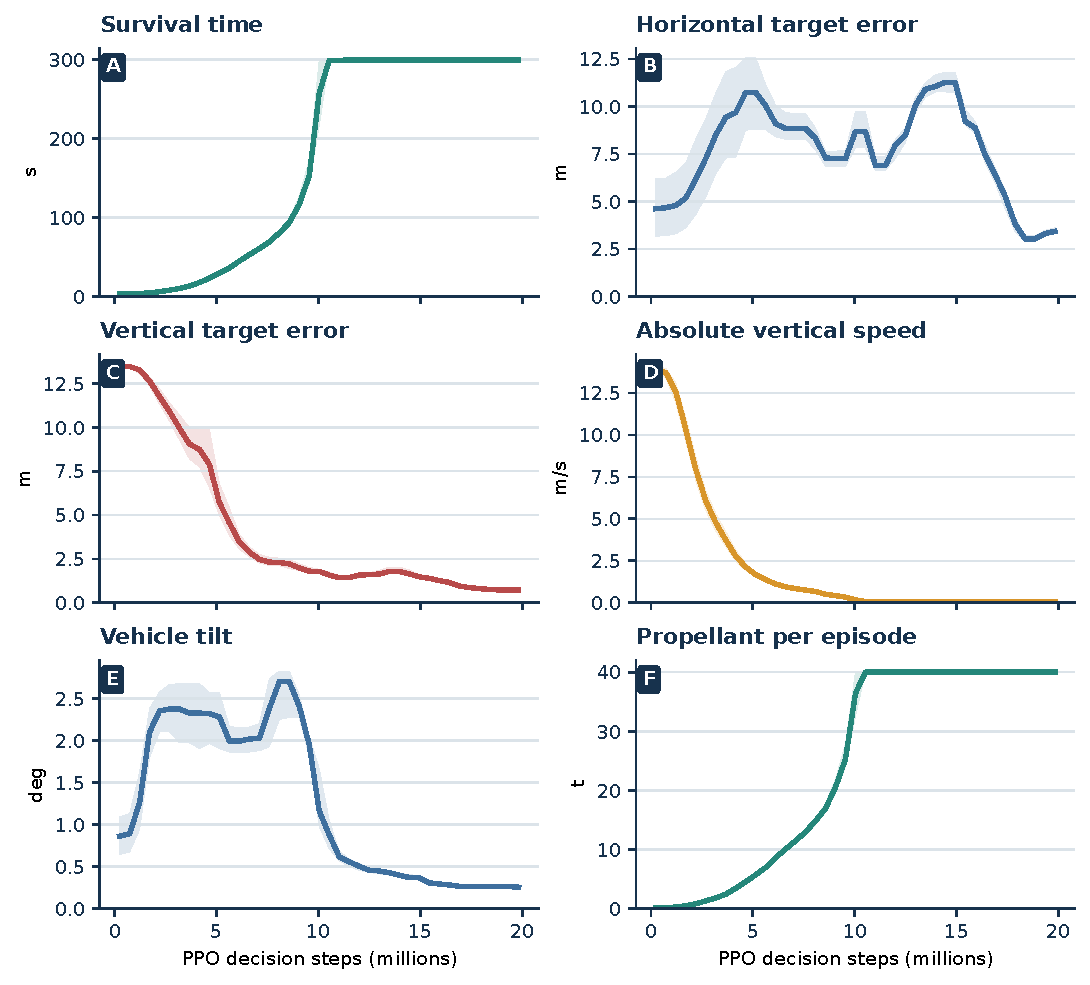
\includegraphics[width=\textwidth]{training/training-hover.pdf}
  \caption{Physical learning curves for \texttt{HoverFixed}. Completed episodes from both
  revisions are ordered chronologically and grouped into 0.5-million-decision-step bins. Lines
  show medians and shading the interquartile range. The final plateau in survival and propellant
  use corresponds to reaching fuel depletion rather than a binary hover-success event.}
  \label{fig:hover-training}
\end{figure}

The complete evaluation confirms the vertical fix under a broader set of initial conditions.
All 250 deterministic trials reached the \SI{60}{s} horizon. They began \SIrange{0.12}{6.61}{m}
from the horizontal target with up to \SI{2.61}{m/s} horizontal speed and
\SI{1.40}{\degree} tilt. Figure~\ref{fig:hover-evaluation} shows the median response and its
interquartile envelope. The commanded descent briefly raises median speed to approximately
\SI{7.5}{m/s}, but vertical error falls from \SI{20}{m} to below \SI{1}{m} and the policy then
damps both translation and attitude. At \SI{60}{s}, median speed is \SI{0.077}{m/s}, median tilt
is \SI{0.105}{\degree} and median vertical error is \SI{0.902}{m}.

\begin{figure}[H]
  \centering
  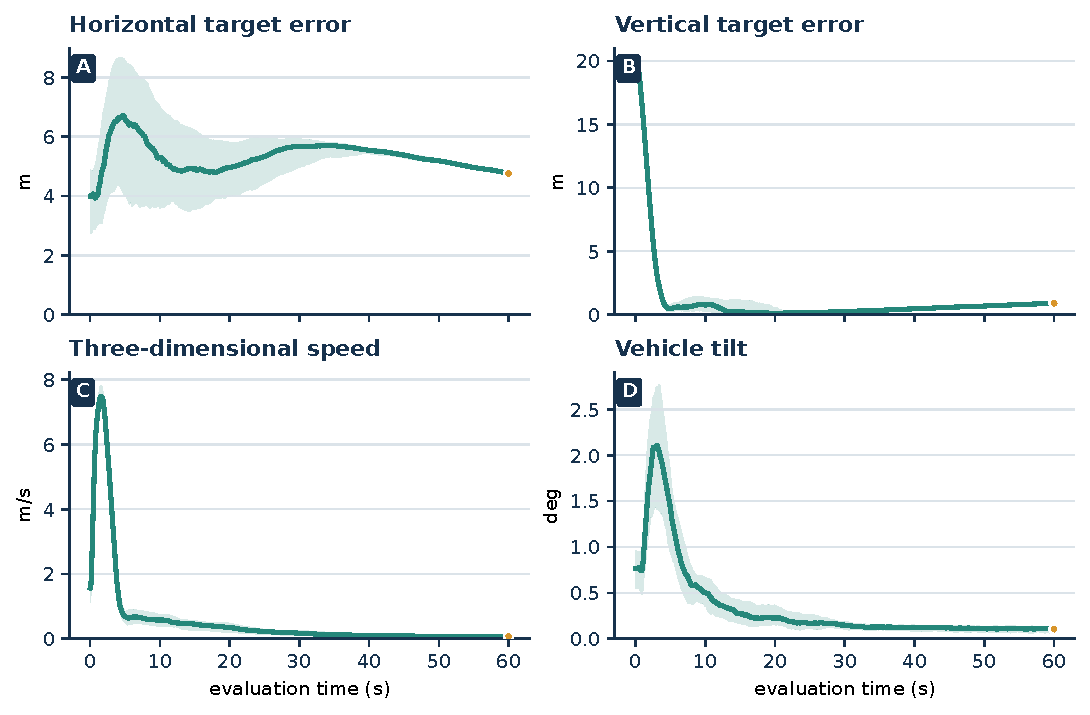
\includegraphics[width=\textwidth]{training/hover-evaluation.pdf}
  \caption{Time-aligned profiles from all 250 \texttt{HoverFixed} evaluation episodes. Lines are
  medians, shaded areas are interquartile ranges and orange markers show the \SI{60}{s}
  endpoints. The policy corrects the initial \SI{20}{m} altitude error and damps motion, but
  converges to a residual horizontal offset.}
  \label{fig:hover-evaluation}
\end{figure}

The terminal means tell the same story: speed \SI{0.073}{m/s}, horizontal speed
\SI{0.066}{m/s}, vertical speed \SI{0.021}{m/s}, tilt \SI{0.100}{\degree} and angular rate
\SI{0.082}{\degree\per\second}. Mean fuel use was \SI{11724.7}{kg}, and only one episode
recorded an engine restart. The remaining weakness is position rather than stability. Horizontal
error first rises, then converges tightly to a median of \SI{4.76}{m}; only 77 of 250 trials end
closer to the target than they began.

These 250 horizon completions are substantially stronger evidence than the previous four-trial
diagnostic, but they are not a 100\% success rate. The evaluator explicitly records that no
binary hover metric is defined. \texttt{HoverFixed} therefore demonstrates repeatable altitude,
velocity and attitude stabilization with a residual planar offset; declaring a solved hover
task requires an acceptance radius chosen before the next evaluation.

\section{Moving-target hover tracking}

Tracking begins where fixed hover ends. The policy must leave a stable state, travel to a new
point and become stable again before the timeout. This makes raw target distance a misleading
learning curve: the relocation radius expands while the policy improves. Figure~\ref{fig:tracking-training}
therefore pairs curriculum progress and success with direction efficiency and settling quality.
Progress rose to 97.6\%, and the binned training-success rate stayed mostly above 80\% after the
initial learning phase. The policy was learning to travel and settle under increasingly difficult
conditions, although none of these training signals is a held-out probability.

\begin{figure}[H]
  \centering
  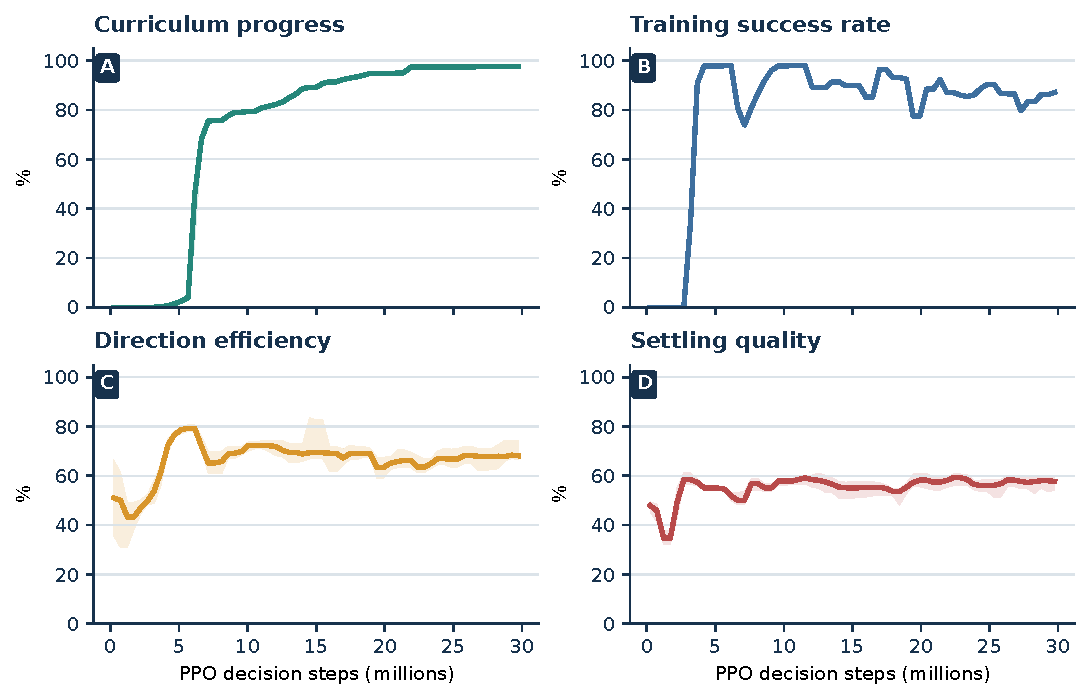
\includegraphics[width=\textwidth]{training/training-hover-track.pdf}
  \caption{Training progression for \texttt{HoverTrackSimple3}. Completed episodes are ordered
  chronologically and grouped into 0.5-million-decision-step bins. Lines show the median and
  shading the interquartile range, except that training success is the bin mean. This view avoids
  mixing repeated episode indices from the three trainer revisions.}
  \label{fig:tracking-training}
\end{figure}

The physical quantities in Figure~\ref{fig:tracking-training-physical} supply the missing
context. Episode duration and propellant use rise as the target moves farther away and the
policy must complete more difficult transfers. Mean horizontal error therefore does not fall in
the same way as it did in fixed hover; after the curriculum expands, it stabilizes despite a
larger task envelope. Horizontal speed peaks during the first attempt to move aggressively, then
settles near \SI{1}{m/s}. Read together with the improving success curve, these are signs of a
controller adapting to a growing problem rather than a stationary metric simply getting worse.

\begin{figure}[H]
  \centering
  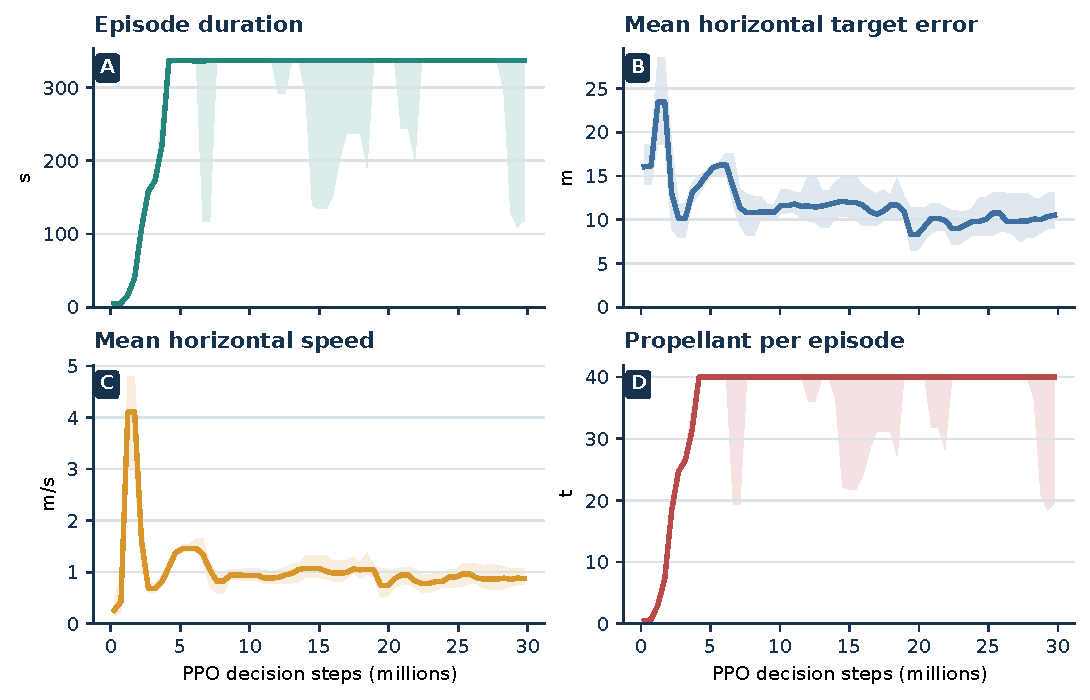
\includegraphics[width=\textwidth]{training/tracking-training-physical.pdf}
  \caption{Physical cost of the expanding \texttt{HoverTrackSimple3} curriculum. Lines are
  binned medians and shaded areas are interquartile ranges. Longer episodes and greater fuel use
  accompany farther target relocations, while speed and horizontal error settle after the early
  learning transient.}
  \label{fig:tracking-training-physical}
\end{figure}

The completed evaluation produced 191 successful episodes out of 250, or 76.4\% with a 95\%
Wilson interval of 70.8--81.2\%. Table~\ref{tab:tracking-bands} gives the exact counts, while
Figure~\ref{fig:tracking-success} shows how the failure appears in time, captures and fuel. The
aggregate number hides a sharp boundary effect: performance was perfect at difficulties 0 and
0.25, 98\% at 0.5, 84\% at 0.75, and 0\% at 1.0.

\begin{table}[htbp]
  \centering
  \caption{\texttt{HoverTrackSimple3} evaluation by curriculum band. Intervals are 95\% Wilson
  intervals; each band contains 50 episodes.}
  \label{tab:tracking-bands}
  \resizebox{\textwidth}{!}{%
  \begin{tabular}{rrrrrr}
    \toprule
    Difficulty & Successes & Rate & 95\% interval & Mean duration (s) & Mean captures \\
    \midrule
    0.00 & 50/50 & 100\% & 92.9--100\% & 31.60 & 3.00 \\
    0.25 & 50/50 & 100\% & 92.9--100\% & 41.43 & 3.00 \\
    0.50 & 49/50 & 98\%  & 89.5--99.6\% & 53.76 & 2.98 \\
    0.75 & 42/50 & 84\%  & 71.5--91.7\% & 74.06 & 2.76 \\
    1.00 & 0/50  & 0\%   & 0.0--7.1\%   & 35.00 & 0.00 \\
    \midrule
    Overall & 191/250 & 76.4\% & 70.8--81.2\% & 47.17 & 2.35 \\
    \bottomrule
  \end{tabular}
  }
\end{table}

\begin{figure}[htbp]
  \centering
  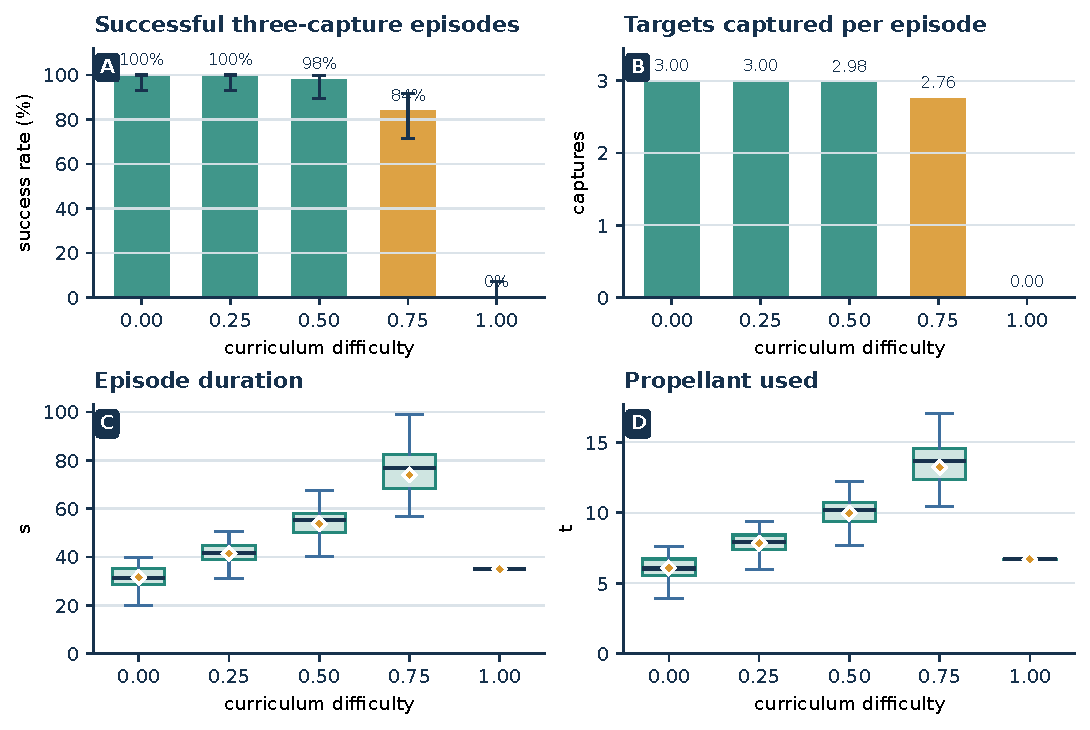
\includegraphics[width=\textwidth]{training/tracking-evaluation.pdf}
  \caption{Fixed-band tracking evaluation. Panel A shows success with 95\% Wilson intervals and
  Panel B the number of completed captures. In Panels C and D, boxes span the interquartile
  range, centre lines are medians, diamonds are means and whiskers extend to \(1.5\) times the
  interquartile range. The exact \(d=1\) boundary produces no captures and a uniform
  \SI{35}{s} timeout.}
  \label{fig:tracking-success}
\end{figure}

Across all bands, mean fuel use was \SI{8759.76}{kg}. Mean final planar distance was
\SI{5.64}{m}; mean final speed was \SI{0.877}{m/s}, composed of
\SI{-0.047}{m/s} vertical and \SI{0.870}{m/s} horizontal velocity. Mean final tilt was
\SI{0.709}{\degree} and angular rate \SI{0.171}{\degree\per\second}. These terminal means mix
successful captures with timeout states and must not be read as capture thresholds.

The full-difficulty failures all ended by target timeout after \SI{35}{s}, with zero captures.
The policy had reached a recorded nonlinear training progress of 97.6\%, but had not actually
trained at an exact, stable 100\% boundary. The abrupt change suggests a curriculum-boundary or
generalization problem. The evidence does not isolate whether the dominant cause is relocation
radius, tightened thresholds, state distribution, insufficient exposure or their interaction;
claiming a specific cause would require controlled evaluations around $d=1$.

The tracking policy therefore learned the complete travel--settle sequence over most of the
tested curriculum, including 84\% success at $d=0.75$, but not at its exact final boundary. This
was the first clear example of training progress and frozen evaluation telling different stories.
Landing keeps the same need to travel and settle, then adds the requirement to do so before
physical contact.

\section{Physical leg landing}

\subsection{Why L10 had to become L11}

L10 established that PPO could learn navigation, braking and stable four-foot support, but its
solution still depended on rapid engine cycling. As that run was continued from 30M to 79.63M
steps, effective curriculum difficulty rose from 12.3\% to 60.2\% while late-window restart count
rose from 10.1 to 23.7. Its fixed-band evaluation then produced 151 successes in 250 episodes and
none at $d=1$. This combination motivated L11: preserve outcome-based rewards, make continuous
one-engine descent physically feasible, and constrain rapid switching.

L11 started from fresh weights and reached the complete curriculum. Figure~\ref{fig:l11-training-progress}
places its learning history beside L10 instead of showing the final run in isolation. Both runs
first learn basic touchdown, but their actuator strategies then separate: L10's median restart
count climbs as its curriculum becomes harder, whereas L11 spends most of training near zero or
one restart while continuing to reduce contact speed. L11 reaches 100\% effective difficulty and
continues improving after the 90M-step resume. In the final 1,000 completed, non-replay episodes
at exact $d=1$, training success was 90.1\%; the saved runtime state's recent counter was 92.9\%.

\begin{figure}[H]
  \centering
  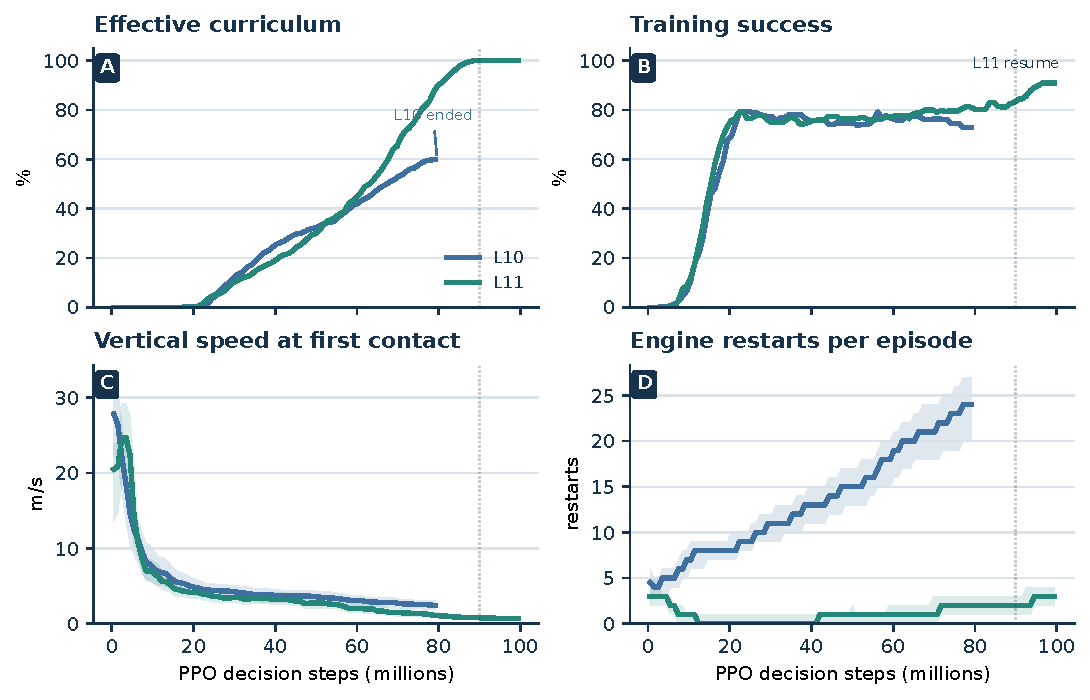
\includegraphics[width=\textwidth]{training/training-leg-landing.pdf}
  \caption{Chronological comparison of L10 and L11, grouped into
  one-million-decision-step bins. Lines are medians with interquartile bands, except that
  training success is a bin mean. Contact speed uses only episodes that reached touchdown. L10
  ends at 79.63M steps; the dotted line marks the L11 resume at 90M. Manifest times isolate the
  intended runs and incomplete shutdown rows are excluded.}
  \label{fig:l11-training-progress}
\end{figure}

The redesign changed more than the success count. Table~\ref{tab:landing-run-comparison} shows
that L11 increased
overall evaluation success by 24.4 percentage points, produced measurable success at exact full
difficulty, and reduced impact and cycling at approximately the same mean fuel use. The restart
reduction is especially large: 18.46 to 1.56 per episode.

\begin{table}[htbp]
  \centering
  \caption{Completed fixed-band landing evaluations. Contact quantities are means over episodes
  that reached touchdown; both evaluations used seed 20257 and 250 episodes.}
  \label{tab:landing-run-comparison}
  \resizebox{\textwidth}{!}{%
  \begin{tabular}{lrr}
    \toprule
    Metric & L10 baseline & L11 final \\
    \midrule
    Final effective curriculum difficulty & 60.25\% & 100\% \\
    Overall success & 151/250 (60.4\%) & 212/250 (84.8\%) \\
    Full-difficulty success & 0/50 (0\%) & 18/50 (36\%) \\
    Mean first-contact vertical speed & \SI{3.02}{m/s} & \SI{1.33}{m/s} \\
    Mean first-contact horizontal speed & \SI{0.70}{m/s} & \SI{0.279}{m/s} \\
    Mean first-contact tilt & \SI{1.54}{\degree} & \SI{0.637}{\degree} \\
    Mean maximum contact impulse & \SI{97.0}{\kilo\newton\second} & \SI{39.1}{\kilo\newton\second} \\
    Mean engine restarts & 18.46 & 1.56 \\
    Mean fuel used & \SI{4590}{kg} & \SI{4529}{kg} \\
    \bottomrule
  \end{tabular}}
\end{table}

Figure~\ref{fig:landing-evaluation-comparison} shows that this was not merely an easier set of
random trials. L10 and L11 used the same seed and the same 50 cases in each band. L11's advantage
widens with difficulty, while its median restart count, vertical contact speed and impact remain
below L10 in every band. The redesign therefore improved both mission completion and the physical
quality of the solution.

\begin{figure}[H]
  \centering
  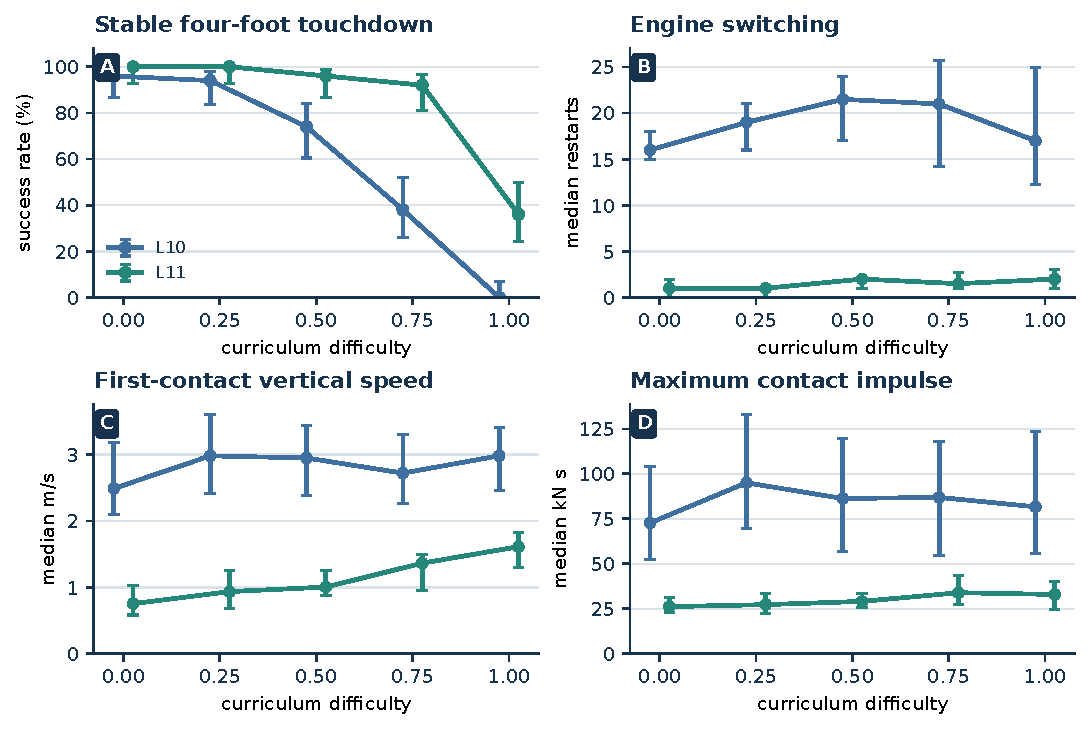
\includegraphics[width=\textwidth]{training/landing-evaluation-comparison.pdf}
  \caption{L10--L11 comparison over the same fixed-band evaluation protocol. Success whiskers
  are 95\% Wilson intervals. The other panels show band medians with interquartile whiskers;
  contact quantities include only episodes that reached touchdown. Lines connect band summaries
  for readability and do not imply interpolation between curriculum levels.}
  \label{fig:landing-evaluation-comparison}
\end{figure}

The final ten million steps produced a smaller net quality gain. Against the same
seeded episode set, overall success rose from 82.8\% at 90M to 84.8\% at 100M, success at
$d=0.75$ rose from 90\% to 92\%, and success at $d=1$ rose from 30\% to 36\%. Mean first-contact
vertical speed fell from \SI{1.68}{m/s} to \SI{1.33}{m/s}, successful-landing planar distance
from \SI{0.97}{m} to \SI{0.63}{m}, and mean maximum impulse from
\SI{52.4}{\kilo\newton\second} to \SI{39.1}{\kilo\newton\second}. At $d=1$, six previously
failing seeded cases succeeded, while three previous
successes regressed. The net gain is real for this fixed set, but the 36\% Wilson interval remains
wide at 24.1--49.9\%.

\subsection{Fixed-band evaluation}

The final evaluation completed all 250 episodes and produced 212 stable four-foot touchdowns:
84.8\% with a 95\% Wilson interval of 79.8--88.7\%. Table~\ref{tab:landing-bands} shows perfect
performance in the first two bands, 96\% at $d=0.5$, 92\% at $d=0.75$, and 36\% at $d=1$.
Figure~\ref{fig:landing-evaluation-comparison} makes the improvement over L10 visible across the
entire range and shows that the gain is accompanied by gentler contact and less switching.

\begin{table}[htbp]
  \centering
  \caption{L11 landing evaluation by fixed curriculum band. Each band contains 50 episodes;
  intervals are 95\% Wilson intervals.}
  \label{tab:landing-bands}
  \resizebox{\textwidth}{!}{%
  \begin{tabular}{rrrrllll}
    \toprule
    Difficulty & Successes & Rate & 95\% interval & Hard touchdown & Missed pad & Too far \\
    \midrule
    0.00 & 50/50 & 100\% & 92.9--100\% & 0 & 0 & 0 \\
    0.25 & 50/50 & 100\% & 92.9--100\% & 0 & 0 & 0 \\
    0.50 & 48/50 & 96\% & 86.5--98.9\% & 1 & 0 & 1 \\
    0.75 & 46/50 & 92\% & 81.2--96.8\% & 2 & 2 & 0 \\
    1.00 & 18/50 & 36\% & 24.1--49.9\% & 30 & 1 & 1 \\
    \midrule
    Overall & 212/250 & 84.8\% & 79.8--88.7\% & 33 & 3 & 2 \\
    \bottomrule
  \end{tabular}}
\end{table}

Across all bands, 248 episodes reached touchdown. Their mean first-contact speed was
\SI{1.38}{m/s}, consisting of \SI{1.33}{m/s} vertical and \SI{0.279}{m/s} horizontal speed;
mean contact tilt was \SI{0.637}{\degree} and angular rate
\SI{1.72}{\degree\per\second}. Mean maximum contact impulse was
\SI{39146}{N.s}, mean rebound was approximately \SI{6.5}{\micro\metre}, and mean recorded stable
hold was \SI{0.566}{s}. No episode recorded a structural strike, one recorded a foot outside the
pad, and every successful episode had all four feet supported. Mean fuel use was \SI{4529}{kg}.

\subsection{Remaining failure and deployment gap}

At full difficulty, 30 of the 32 failures were hard touchdowns; every one exceeded the
\SI{1.5}{m/s} vertical-speed limit. In 25 of those 30 cases, vertical speed was the only failed
first-contact condition, and ten were within \SI{0.2}{m/s} of passing. Median touchdown vertical
speed improved from \SI{1.745}{m/s} at 90M to \SI{1.612}{m/s} at 100M. The remaining problem is
therefore usually a narrow final-braking margin rather than the broad navigation failure seen in
L3--L7. Figure~\ref{fig:landing-full-difficulty} shows both that concentration near the vertical
threshold and the two rare, much larger excursions.

\begin{figure}[H]
  \centering
  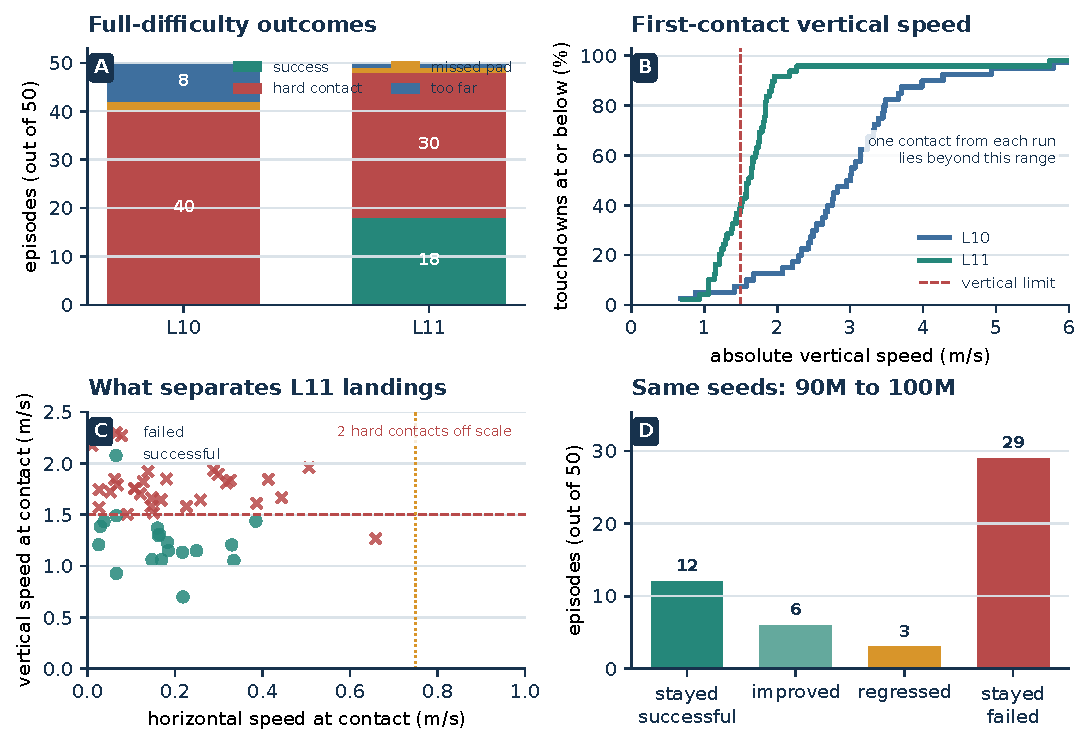
\includegraphics[width=\textwidth]{training/landing-full-difficulty.pdf}
  \caption{Diagnostics at exact full difficulty. Panel A separates the 50 outcomes per run;
  Panel B gives empirical cumulative distributions of contact vertical speed, zoomed to
  \SIrange{0}{6}{m/s}; Panel C zooms into L11's touchdown threshold region, with two hard
  contacts outside the displayed range; and Panel D pairs the same 50 seeds at 90M and 100M.
  The dashed red lines mark the \SI{1.5}{m/s} vertical limit and the dotted amber line marks the
  \SI{0.75}{m/s} horizontal limit.}
  \label{fig:landing-full-difficulty}
\end{figure}

The larger unresolved issue is the difference between training and deployment. Exact-$d=1$
training success was 89.6\% over the final 5,000 completed non-replay episodes and 90.1\% over the
final 1,000, yet deterministic evaluation succeeded in only 36\%. Incomplete curriculum exposure
cannot explain this gap because L11 reached and remained at full difficulty.

The action interface is a plausible, but not yet proven, cause. PPO explores with stochastic
continuous actions during training, whereas the evaluator requests deterministic inference. The
three engine-enable commands are nevertheless encoded as continuous outputs and converted to
binary state through on/off thresholds of $+0.35$ and $-0.35$. A deterministic mean action can
therefore occupy the dead band or switch differently from sampled training actions. Consistent
with that hypothesis, mean restarts rose from 1.32 to 1.56 overall and from 2.02 to 2.46 at
$d=1$ between 90M and 100M, even as touchdown quality improved. The decisive follow-up is an
A/B evaluation of the same checkpoint and seeds with deterministic inference enabled and
disabled, followed by a discrete or hybrid engine-enable action if the gap persists.

The bounded result is still substantial: L11 controls navigation, descent, final flare and
stable support reliably through $d=0.75$, and it completes more than one third of trials at the
full trained boundary. It is not a flight controller or a solved full-difficulty policy.

\section{Answers to the research questions}

Taken together, the three tasks answer the research questions at different levels. For RQ1, the
snapshot, derived policy schema, immutable revisions, telemetry and evaluator form a complete
path from a configurable Unity experiment to an identifiable result.

For RQ2, PPO produced repeatable fixed-hover stabilization across 250 trials, although a
predeclared success rule and tighter planar position hold are still missing. It completed
moving-target tracking reliably through $d=0.75$ and learned physical four-leg landing across
the complete curriculum. The final landing policy still fell to 36\% success at $d=1$, so
reaching full training difficulty did not make the controller uniformly reliable.

For RQ3, the decisive failures formed the same chain as the simulator's development: reward
accumulation encouraged delay or cheap termination; a spawn-order bug removed the requested
initial velocity; incorrectly balanced terms made crashing cheaper than missing; approximate
aerodynamics produced wrong or excessive forces; and implicit UI and policy contracts made
changes difficult to trace. The architecture is largely the record of how those failures were
made observable and prevented from recurring.

\chapter{Limitations and Future Work}
\label{ch:limitations}

Each successful stage of the project narrowed the remaining uncertainty. The simulator can now
configure, train, replay and evaluate substantially different control tasks, and the evaluated
policies have measurable operating ranges. The results do not establish a flight-ready
controller, superiority of PPO or robustness to every option visible in the UI. The remaining
work follows from three boundaries: the world being simulated, the experiments performed inside
it, and the software used to preserve them.

\section{Boundary of the physical model}

The physical model became more complete as new components required it, but it remains a
six-degree-of-freedom rigid body with configurable low-order forces. It does not include
propellant slosh, elastic structure, detailed engine transients, plume--ground interaction,
compressible or transonic aerodynamics, resolved grid-fin lattice flow, sensor noise or
realistic turbulent wind. Pressure-dependent thrust and specific impulse are approximations,
and landing contact is resolved by Unity colliders and a general-purpose solver. No flight data
or independent high-fidelity simulator validates the trajectory as a whole.

The measured policy performance is consequently valid inside the documented simulator. The
next useful physics step is not to add every missing effect at once. It is to determine which
current approximation changes the control outcome. Analytical force cases, published
aerodynamic data and comparison with a higher-fidelity tool could quantify coefficient
sensitivity before additional complexity is introduced.

\section{Boundary of the experiments}

Every completed result uses one principal training seed, one network architecture and one PPO
configuration. Wilson intervals describe repeated episodes for a fixed model; they do not
measure how much performance would vary across independently trained policies. Using one common
evaluation seed makes the five-band studies repeatable, but still samples only one deterministic
set of initial conditions.

The two curriculum tasks also fail differently at their hardest boundary. Tracking falls from
84\% success at $d=0.75$ to zero at $d=1$ after training stopped short of a stable full-difficulty
distribution. L11 landing trained at $d=1$ but achieved only 36\% there during deterministic
evaluation. These results lead to different next experiments. Tracking should be evaluated more
densely between $d=0.75$ and $d=1$ and trained with explicit probability mass at the boundary.
Landing should keep the final checkpoint and seeds fixed while changing only deterministic
versus stochastic inference.

If that landing comparison reproduces the training--evaluation gap, the next design change
should target the action interface rather than the reward. Engine enable is physically binary
but is currently produced by a thresholded continuous output. A discrete branch, or a deliberate
hybrid action space, would remove the dead band between the on and off thresholds. Only after
that isolated test should the main runs be repeated across several trainer and evaluator seeds.

Fixed hover now has a complete 250-episode evaluation, but still lacks a predeclared binary
criterion. The new policy corrects the earlier vertical drift and consistently damps velocity
and attitude, yet converges to a mean final planar offset of \SI{4.77}{m}. The next hover
experiment should define its acceptance radius and hold time before execution, then determine
whether the offset comes from reward balance, observations or the learned equilibrium.

The reward system has a related boundary. Configurability makes a specification inspectable but
does not make it correct. A future validator could estimate the maximum cumulative contribution
of every continuous term and warn when waiting can dominate a terminal outcome. Scripted
adversarial policies---prolonged hovering, engine-off descent and deliberate early
termination---could test these economics before an expensive training run begins.

\section{Boundary of the software product}

Architecture had to evolve while scenes, prefabs, sessions and ONNX policies already existed.
The current schema checks protect known interfaces, but they cannot guarantee migration of every
legacy artifact. Some agent partial classes remain large, not every UI path has an automated
test, and the final public commit is not yet frozen.

A command-line experiment runner would be the most useful complement to the interactive UI. It
could queue matrices of seeds and configurations without manual setup and make larger comparisons
less error-prone. Automated edit- and play-mode tests, a dependency lock, a small known-answer
evaluation and an explicit artifact migration tool would then make the public release easier to
verify and maintain.

\section{A deliberate order for future experiments}

The simulator exposes many possible extensions, but repeating the original scope problem would
make their results difficult to interpret. The next work should therefore proceed in the order
in which each experiment unlocks the next:

\begin{enumerate}
  \item define fixed-hover acceptance limits, diagnose its planar offset and isolate the L11
  deterministic-inference gap;
  \item repeat the principal policies across several seeds once their protocols are stable;
  \item compare selected vehicle configurations on one frozen task, retraining whenever the
  policy interface changes;
  \item measure a no-wind policy under controlled wind, then compare it with a policy trained
  through domain randomization;
  \item inject one actuator fault at a time with fixed onset, duration and severity before
  attempting combined faults; and
  \item treat tower-arm capture as a separate task with its own contact model and evaluation.
\end{enumerate}

This order keeps the core claim modest: the current thesis demonstrates the configurable
workflow and three control tasks. Wind, faults, vehicle comparisons and tower capture remain the
next chapters of the product rather than unevaluated additions to the present result.

\section{Final thesis completion checklist}

\begin{thesistodo}
  Run the deterministic/stochastic L11 inference diagnostic; declare hover acceptance limits
  and diagnose its planar offset;
  freeze and publish the repository revision; add UI/task screenshots and seed-labelled videos;
  translate the approved text to Slovene; insert the official STUDIS description, mentor titles,
  acknowledgements and student email; update both abstracts after the final accepted results;
  and have the mentor approve the final title and scope.
\end{thesistodo}

\chapter{Conclusion}
\label{ch:conclusion}

This thesis began with a simple question: could reinforcement learning make a simulated booster
land? The first cylinder showed that it could, but it also made the question less interesting.
With an oversized engine, constant mass and no aerodynamics, a successful landing said little
about how the controller would behave when the vehicle changed. The project therefore became an
attempt to build the experiment around the policy, not only the policy itself.

That change in focus explains the final simulator. Vehicle hardware, physical parameters,
objectives, curricula, learning settings, faults and telemetry can all be configured through one
workflow. Editable values become immutable sessions before training starts. Observation and
action dimensions follow the selected hardware, incompatible models are rejected, and every
continuation creates a traceable revision. These mechanisms grew out of practical failures: a
configuration panel made shared state ambiguous, modular hardware broke manually maintained
policy dimensions, and resumed runs needed to preserve rather than overwrite their history.

The three tasks then tested the system at increasing levels of difficulty. The revised fixed-hover
policy completed all 250 \SI{60}{s} horizons, reducing terminal speed to \SI{0.073}{m/s} and
tilt to \SI{0.100}{\degree}, although its \SI{4.77}{m} mean planar offset and the absence of a
binary criterion prevent a success-rate claim. Moving-target hover completed 191 of 250
deterministic trials and remained reliable through $d=0.75$, before failing at the exact
curriculum boundary. The final L11 landing policy completed 212 of 250 trials,
including 18 of 50 at $d=1$. Compared with L10, it reduced mean engine restarts from 18.46 to
1.56 and mean first-contact vertical speed from \SI{3.02}{m/s} to \SI{1.33}{m/s}. The policy
learned navigation, braking, engine sequencing and stable four-foot support, although its 36\%
full-difficulty success shows that the final boundary is not solved reliably.

The L1--L11 campaign explains how that result was reached. A policy that appeared to fly away
revealed a missing spawn velocity. A policy that reached the pad and crashed revealed a capped
impact penalty. Frequent contact revealed that one foot was not a landing, and a policy that
learned with easier actuators revealed excessive engine cycling. Each failure made the next
question narrower. Telemetry and component tests were what turned surprising behaviour into a
specific change to physics, reward, termination, actuation or software ownership.

The central lesson is that an RL policy learns the environment it receives, including its
mistakes. More reward terms do not necessarily express intent more accurately, and more physical
detail does not automatically make an experiment trustworthy. The useful combination is an
explicit model, rewards whose contributions can be inspected, clear ownership of state and an
evaluation that remains separate from training.

The final deterministic landing gap is therefore not an inconvenient result to hide; it is the
next question exposed by the system. A matched stochastic-inference test can determine whether
the continuous representation of binary engine-enable actions contributes to that gap. The
hover task similarly turns its residual planar offset into a specific next test: freeze an
acceptance radius and hold time, then change one suspected cause at a time. Later studies can add
vehicle comparisons, wind and faults under the same discipline. The project has moved from
making one object land to building a product in which the reason it landed---or failed to
land---can be examined.


\appendix
\chapter{Reproducibility Record}
\label{app:reproducibility}

The development chapters explain why each experiment changed. This appendix provides the other
half of that story: the identifiers needed to trace each reported number back to a saved run.

\section{Software environment}

\begin{table}[htbp]
  \centering
  \caption{Recorded software and hardware environment for the completed runs.}
  \begin{tabular}{ll}
    \toprule
    Component & Version or value \\
    \midrule
    Unity Editor & 6000.4.1f1 \\
    Unity ML-Agents package & 4.0.2 \\
    Python & 3.10.12 \\
    ML-Agents Python package & 1.1.0 \\
    PyTorch & 2.1.0+cu121 \\
    CUDA runtime & 12.1 \\
    GPU & NVIDIA GeForce RTX 4070 SUPER \\
    Physics timestep & \SI{0.01}{s} \\
    Decision period & 3 physics steps \\
    \bottomrule
  \end{tabular}
\end{table}

\section{Run identifiers}

\begin{description}
  \item[Hover training] \texttt{HoverFixed}, revision 2, 20,078,171 steps,
  environment seed 1, trainer seed 1, evaluated export \texttt{Rocket.onnx}.
  \item[Hover evaluation] completed 2026-09-03, seed 20257, 250 episodes,
  summary \path{telemetry_HoverFixed_evaluation_20260903_134045_summary.json}.
  \item[Tracking training] \texttt{HoverTrackSimple3}, revision 3, 30,000,039 steps,
  environment seed 1, trainer seed 1.
  \item[Tracking evaluation] completed 2026-08-24, seed 20257, 250 episodes,
  summary \path{telemetry_HoverTrackSimple3_evaluation_20260824_192643_summary.json}.
  \item[Landing baseline] \texttt{L10}, revision 4, 79,629,752 steps; evaluation completed
  2026-08-31 with seed 20257 and 250 episodes,
  summary \path{telemetry_L10_evaluation_20260831_191953_summary.json}.
  \item[Landing training] \texttt{L11}, revision 2, 100,000,086 steps, environment seed 1,
  trainer seed 1, evaluated export \texttt{Rocket.onnx}.
  \item[Landing evaluation] completed 2026-09-02, seed 20257, 250 episodes,
  summary \path{telemetry_L11_evaluation_20260901_235641_summary.json}.
\end{description}

\begin{thesistodo}
Repository URL: TODO. Final commit: TODO. The present Git HEAD is not a valid substitute because
the simulator working tree contains uncommitted changes. Add final tracking and hover hashes;
the L11 landing hashes are recorded in Appendix~\ref{app:landing}.
\end{thesistodo}

\section{Artifact layout}

The record closes the experimental loop only if the underlying files are kept together. For each
run, the public artifact should preserve \texttt{RunManifest.json}, \texttt{RuntimeState.json},
all numbered revisions, trainer logs, discussed checkpoints, the final ONNX model, the evaluation
episode CSV and its summary JSON. The README should then describe the command or UI sequence used
to load the session and repeat the evaluation.

\chapter{Landing Experiment Record}
\label{app:landing}

The main text follows L11 as the final step in the landing campaign. This appendix gathers its
identity, configuration and outcome in one place so that the narrative can be checked against the
immutable artifacts. Repository identity remains a submission placeholder until the working tree
is frozen for publication.

\newcommand{\hashvalue}[4]{\begingroup\ttfamily\footnotesize#1\hspace{0pt}#2\hspace{0pt}#3\hspace{0pt}#4\endgroup}
\small
\begin{longtable}{p{0.38\textwidth}p{0.52\textwidth}}
  \toprule
  Field & Value \\
  \midrule
  \endhead
  Run ID and revision & \texttt{L11}, revision 2 (continuation of the same run from 90M to 100M) \\
  Repository commit & TODO after final source freeze \\
  Manifest session identity & \hashvalue{438cf2baccfafe0f}{0a924bf61021a88d}{eb3515c33e74d9d3}{871f539338888deb} \\
  Raw revision-2 \texttt{Session.json} SHA-256 &
  \hashvalue{c166eb67f9b0e810}{b8d40b43b8f0f17f}{33290e4d41119b6a}{bc7bccbf36f45a40} \\
  Model SHA-256 &
  \hashvalue{e03b8facb32a0c40}{ee9449625767d6b4}{315965450028ec3a}{c8f511c8b344830b} \\
  Evaluation-summary SHA-256 &
  \hashvalue{fd48f2dc02351a0c}{752853939ee04b4c}{a267ff0d36df9f59}{796922b3828e329d} \\
  Reward preset/version & Balanced, objective schema 16; success-only mission efficiency \\
  Trainer/environment seeds & 1 / 1 \\
  Training steps and revisions & 100,000,086; two immutable revisions \\
  Final curriculum progress & 100\% linear and effective; 92.90\% recent success \\
  Policy interface & 52 observations; 12 continuous actions; three independent engines \\
  Evaluated model & \texttt{Rocket.onnx}, final checkpoint 100,000,086 \\
  Evaluation seed and episode count & 20257; 250 (50 per fixed difficulty band) \\
  Stable four-foot touchdown rate (95\% CI) & 212/250 = 84.8\% (79.8--88.7\%) \\
  Full-difficulty touchdown rate (95\% CI) & 18/50 = 36\% (24.1--49.9\%) \\
  First-contact speed, vertical/horizontal & \SI{1.38}{m/s}; \SI{1.33}{m/s} / \SI{0.279}{m/s}
  over 248 touchdown episodes \\
  First-contact tilt and angular rate & \SI{0.637}{\degree}; \SI{1.72}{\degree\per\second} \\
  Maximum impulse and rebound & mean maximum \SI{39146}{\newton\second}; mean maximum
  \SI{6.55}{\micro\metre} \\
  Stable-hold time & mean \SI{0.566}{s} \\
  Structural-strike rate & 0/250 = 0\% \\
  Foot-outside-pad rate & 1/250 = 0.4\% \\
  Engine use & mean 3.00 first ignitions and 1.56 restarts per episode \\
  Fuel used & mean \SI{4529}{kg} over all evaluation episodes \\
  Dominant failure modes & 33 hard touchdowns, 3 missed-pad and 2 too-far terminations; 30 hard
  touchdowns occurred at full difficulty \\
  \bottomrule
\end{longtable}
\normalsize

The evaluation-summary file reports \texttt{aborted: false}. No wind, fins, RCS or injected
faults were active. L11 used minimum throttle 0.499, startup delay \SI{0.45}{s}, shutdown
transient \SI{0.20}{s}, minimum run \SI{1.5}{s}, cooldown \SI{2.0}{s} and throttle spool rate
5.8 per second. Its success-only efficiency magnitude, restart equivalent and touchdown-quality
fraction were increased relative to L10 to favour longer useful burns without making early
shutdown attractive on failed episodes.

The full-difficulty result is based on a model trained at 100\% curriculum, but it remains much
lower than exact-$d=1$ training success. This discrepancy is retained as a finding rather than
removed through checkpoint selection. The next controlled diagnostic is the deterministic versus
stochastic inference comparison described in Chapter~\ref{ch:limitations}.

Before submission, add representative seed-labelled success and failure videos and the final
public repository commit. Video remains qualitative evidence; the numeric result above comes
from the complete evaluation summary.


\printbibliography[heading=bibintoc,title={References}]
\end{document}
